% GO TO: /Users/leonlufkin/Library/texmf/tex/latex
%        to add custom packages to the path
\documentclass{article}
\usepackage{report}

\title{Receptive Field Localization}
\author{Leon Lufkin}
\date{\today}

\makeatletter
\let\Title\@title
\let\Author\@author
\let\Date\@date

\begin{document}

%%%%%%%%%%%%%%%%%
%% The Problem %%
%%%%%%%%%%%%%%%%%
\section{The Problem}
We consider a feedforward neural network with a single hidden layer and activation function $\sigma$.
It receives an input $x \in \R^n$ and produces a scalar output $\hat{y} \in \R$.
The hidden layer has $K$ units.
The weights for the first and second layer are $W_1 \in \R^{K \times n}$ and $W_2 \in \R^{1 \times K}$, respectively, and the corresponding biases are $b_1 \in \R^K$ and $b_2 \in \R$.
\begin{align}
  \hat{y} &= W_2 \sigma( W_1 x + b_1 ) + b_2. \label{eq:model}
\end{align}

Our data $x$ are sampled from a mixture of two translation-invariant distributions in some family $\{ p_\xi \}_{\xi}$ parameterized by a correlation length-scale $\xi$.
That is, we sample $x \sim p_{\xi_1}$ with probability $\frac{1}{2}$ and $x \sim p_{\xi_2}$ otherwise.
If $x$ is sampled from $p_{\xi_1}$, then $y(x) = 1$; otherwise, $y(x) = 0$. 
We can train using either mean-squared error or cross-entropy loss, though we primarily consider the former. 

Alessandro's paper primarily considers the case where $W_2 = \frac{1}{K} \mathbf{1}^\top$ (take the mean of the hidden activations) is fixed and $\sigma(h) = \text{erf}(\frac{h}{\sqrt{2}})$.
I have also tried $\sigma = \text{sigmoid}, \text{ReLU}$.
For the former, the results are qualitatively identical, while for the latter we get localization if $\xi_1 > \xi_2$ and short-range oscillations otherwise.
For $\sigma = \text{ReLU}$, one can further remove the bias terms $b_1$ and $b_2$ (though not for sigmoid).
% TODO: explain why

We consider two types of datasets: the nonlinear Gaussian process (NLGP) and the single pulse (SP).
We explain them in more detail later.
They differ primarily in that the former has continuous support on $\R^n$, while the latter has discrete support on a subset of $\{ 0, 1 \}^n$.
The former also has a gain parameter that controls the degree of localization, while the latter does not. 

\emph{We'll present the results in reverse order, since it makes more sense logically.
We start by attempting to analyze the ReLU model directly.
This will force us to assume Gaussian data, which captures only half of what we'd like to describe.
We will discuss some ideas about how to extend this to the non-Gaussian case, and perhaps also the SP dataset.}

\emph{To address these analytical roadblocks, we'll explore using a gated deep linear network (GDLN) to model the ReLU network.
This will require some assumptions about the gating structure, which we test empirically.
However, we're not really sure how to properly set up the ``neural race'' and map the winner onto the ReLU case.
We consider a few approaches, though we are not sure which is correct.
We'll conclude with some questions, concerns, and ideas, with specific focus on the discrete Fourier transform, uncertainty principle, and characteristic functions.}


%%%%%%%%%%%%%%%%%%%
%% ReLU Analysis %%
%%%%%%%%%%%%%%%%%%%
\section{ReLU Analysis}
Let's start by trying to analyze the gradient flow for a ReLU network.
We won't be able to solve it exactly, but we can get some intuition.
We will have to assume the data are Gaussian to say something interesting after just a few steps.
Of course, this is the case we are less interested in, since it's the non-Gaussian data that shows localization.

Let $w_i$ be the $i$-th row in $W_1$.
We make predictions with
\begin{align}
  \hat{y}(x) &= \frac{1}{K} \sum_{k \in [K]} \text{ReLU}(\langle w_k, x \rangle).
\end{align}
We use MSE loss,
\begin{align}
  \LL &= \frac{1}{2} \E_{X,Y} \left[ \left( \hat{y}(X) - Y \right)^2 \right].
\end{align}
The corresponding gradient flow for $w_1$ is given by
\begin{align}
  \tau \frac{d}{dt} w_1
  &= -\E_{X,Y} \left[ \left( \frac{1}{K} \sum_{k \in [K]} \text{ReLU}(\langle w_k, X \rangle) - Y \right) \frac{\partial}{\partial w_1} \left[ \text{ReLU}(\langle w_1, X \rangle) \right] \right] \\
  &= \frac{1}{2} \E_{X, \langle w_1, X \rangle > 0 \mid Y=1} \left[ X \right] - \frac{1}{K} \sum_{k \in [K]} \E_{X,Y, \langle w_1, X \rangle > 0, \langle w_k, X \rangle > 0} \left[ \langle w_k, X \rangle X \right]
\end{align}

%%%%%%%%%%%%%%%%%%%
%% Gaussian Data %%
\subsection*{Gaussian Data}
To compute these conditional expectations, we will have to assume the data are Gaussian.
% (Below, I try to do this without assuming Gaussian data, but I haven't been able to make any meaningful progress there yet.)
We begin by computing the first conditional expectation.
Define the random variable $S = \langle w_1, X \rangle$.
\begin{align} \label{eq:yx_cond_exp}
  \E_{X, S > 0 \mid Y=1} \left[ X \right]
  &= \E_{S > 0 \mid Y=1} \left[ \E_{X \mid S, Y=1} \left[ X \right] \right].
  % \PR\left( S > 0 \mid Y = 1 \right).
\end{align}
Let us consider $X$ sampled from $p_{\xi_1}$ (i.e. with label $Y=1$) and write
\begin{align}
  X &= AX + S v, \label{eq:X_rewrite}
\end{align}
where
\begin{align}
  v &= \frac{1}{ w_1^\top \Sigma_1 w_1 } \Sigma_1 w_1, \\
  A &= I_n - v w_1^\top.
\end{align}
\Cref{eq:X_rewrite} clearly holds.
Our specific selection of $v$ and $A$ guarantees that $A X$ and $S$ have zero covariance.
\emph{Since $X$ is Gaussian, this implies they are independent.}
So, $X \mid S \sim \NN\left( S v, A \Sigma A^\top \right)$.
Note that $\E_{S \mid S>0, Y=1} \left[ S \right] = \left( \frac{2}{\pi} w_1^\top \Sigma_1 w_1 \right)^{\frac{1}{2}}$.
Plugging this into \cref{eq:yx_cond_exp},
\begin{align}
  \E_{X, S > 0 \mid Y=1} \left[ X \right]
  &= \E_{S>0 \mid Y=1} \left[ S v \right] \\
  &= \E_{S \mid S>0, Y=1} \left[ S v \right] \PR\left( S > 0 \mid Y = 1  \right) \\
  % &= \frac{1}{2} \left( \frac{2}{\pi} w_1^\top \Sigma_1 w_1 \right)^{\frac{1}{2}} \frac{1}{ w_1^\top \Sigma_1 w_1 } \Sigma_1 w_1 \\
  &= \frac{1}{\sqrt{2 \pi}} \left( w_1^\top \Sigma_1 w_1 \right)^{-\frac{1}{2}} \Sigma_1 w_1.
\end{align}

Now, let us evaluate the second conditional expectation.
First, we consider the case $k=1$.
Then, we only have one positivity constraint.
We use $S$ again, just as before.
Let us also only consider $X$ with label $Y=1$.
Both labels appear in the ODE for this term, but the result has the same form.
\begin{align} \label{eq:xx_w1_cond_exp}
  \E_{X, S > 0 \mid Y=1} \left[ S X \right]
  &= \E_{S > 0 \mid Y=1} \left[ S \E_{X \mid S, Y=1} \left[ X \right] \right] \PR( S > 0 \mid Y = 1  )
  = \E_{S \mid S > 0, Y=1} \left[ S^2 \right] v \PR( S > 0 \mid Y = 1 ).
\end{align}
By symmetry of $S$ about 0, $\E_{S \mid S > 0, Y=1} \left[ S^2 \right] = \E_{S \mid Y=1} \left[ S^2 \right] = w_1^\top \Sigma_1 w_1$.
(This step does not require Gaussianity!)
So,
\begin{align}
  \E_{X,\langle w_1, X \rangle > 0 \mid Y=1} \left[ \langle w_1, X \rangle X \right]
  &= \frac{1}{2} w_1^\top \Sigma_1 w_1 \left( \frac{1}{ w_1^\top \Sigma_1 w_1 } \Sigma_1 w_1 \right)
  = \frac{1}{2} \Sigma_1 w_1.
\end{align}

Now, let us consider $k>1$.
We will need to consider both positivity constraints.
This is going to get really messy!
I will skip the analysis here and just present the final result.
(See an earlier version of this document for all the steps.)

We'll need to define some more variables to make things a bit more compact.
\begin{align}
  \rho_{ij} &= w_i^\top \Sigma w_j \qquad \text{for $i,j = 1,k$}
  \qquad \text{and} \qquad
  \gamma = \frac{ \rho_{1k} }{ \sqrt{ \rho_{11} \rho_{kk} } }.
\end{align}
In toto,
\begin{align}
  &\E_{X, \langle w_1, X \rangle > 0, \langle w_k, X \rangle > 0 \mid Y=1} \left[ \langle w_k, X \rangle X \right] \\
  &\begin{multlined} = \left[ \frac{1}{2\pi (1 - \gamma^2) } \left( \frac{ \rho_{kk} }{ \rho_{11} } \cos^{-1}(-\gamma) - \gamma^2 \sin^{-1}(\gamma) \right) 
    + \frac{ \frac{1}{\gamma \rho_{11}} - \frac{1}{\sqrt{ \rho_{11}\rho_{kk} }} }{ 2\pi \sqrt{1-\gamma^2} }
     \right] \Sigma_1 w_1  \\
    + \left[ -\frac{ \gamma }{2\pi (1 - \gamma^2) } \sqrt{\frac{\rho_{11}}{\rho_{kk}}} \left( \frac{\rho_{kk}}{\rho_{11}} \cos^{-1}(\gamma) - \sin^{-1}(\gamma) \right)
    + \frac{ \frac{1}{ \gamma \rho_{kk} } - \frac{1}{ \sqrt{ \rho_{11}\rho_{kk} }  }  }{ 2\pi \sqrt{1-\gamma^2} }
    \right] \Sigma_1 w_k
  \end{multlined} \\
  &\begin{multlined} = \left[ \frac{\gamma^{2}-\frac{\rho_{kk}}{\rho_{11}}}{2\pi(1-\gamma^{2})}\cos^{-1}\left(\gamma\right)+\frac{2\frac{\rho_{kk}}{\rho_{11}}-\gamma^{2}}{4(1-\gamma^{2})}+\frac{\frac{1}{\gamma\rho_{11}}-\frac{1}{\sqrt{\rho_{11}\rho_{kk}}}}{2\pi\sqrt{1-\gamma^{2}}} \right] \Sigma_1 w_1  \\
    + \left[ \text{? some mess ?} \right] \Sigma_1 w_k
  \end{multlined}
\end{align}

\paragraph*{A single neuron}
Let's consider what happens if we have just one hidden neuron, i.e. $K=1$.
Then, the above analysis simplifies greatly.
The gradient flow becomes
\begin{align}
  \tau \frac{d}{dt} w_1
  &= \frac{1}{2} \E_{X, \langle w_1, X \rangle > 0 \mid Y=1} \left[ X \right] - \E_{X,Y, \langle w_1, X \rangle > 0} \left[ \langle w_1, X \rangle X \right] \\
  % &= \frac{1}{2 \sqrt{2 \pi}} \left( w_1^\top \Sigma_1 w_1 \right)^{-\frac{1}{2}} \Sigma_1 w_1 - \frac{1}{4} \left( \Sigma_0 + \Sigma_1 \right) w_1 \\
  &= - \frac{1}{4} \left( \Sigma_0 + \left( 1 - \sqrt{\frac{2}{\pi}} \left( w_1^\top \Sigma_1 w_1 \right)^{-\frac{1}{2}} \right) \Sigma_1 \right) w_1.
\end{align}
Recall that both $\Sigma_0$ and $\Sigma_1$ are circulant, so they diagonalize in the discrete Fourier transform basis.
(Actually, since they are real, symmetric matrices, they diagonalize in the discrete sine/cosine transform basis.)
Let us analyze $w_1$ in this basis by defining $u_1 = F^\top w_1$, where $F$ is the discrete sine/cosine transform matrix.
Let $\Lambda_0$ and $\Lambda_1$ be the diagonal matrices of eigenvalues for $\Sigma_0$ and $\Sigma_1$, respectively.
Then,
\begin{align}
  \tau \frac{d}{dt} u_1
  &= - \frac{1}{4} \left( \Lambda_0 + \left( 1 - \sqrt{\frac{2}{\pi}} \left( u_1^\top \Lambda_1 u_1 \right)^{-\frac{1}{2}} \right) \Lambda_1 \right) u_1.
  \label{eq:grad_flow_K1_diag}
\end{align}
\Cref{fig:K1_receptive_fields} establishes the validity of \cref{eq:grad_flow_K1_diag} for Gaussian data.
(Note the empirical and theoretical receptive fields are slightly different because the former uses minibatches while the latter uses the full dataset, and also because of a possible slight issue with learning rates.
If both of these are extended to infinity, they align almost perfectly, but I wanted to show the evolution as well.)

\begin{figure}
  \centering
  \begin{tabular}{ccc}
    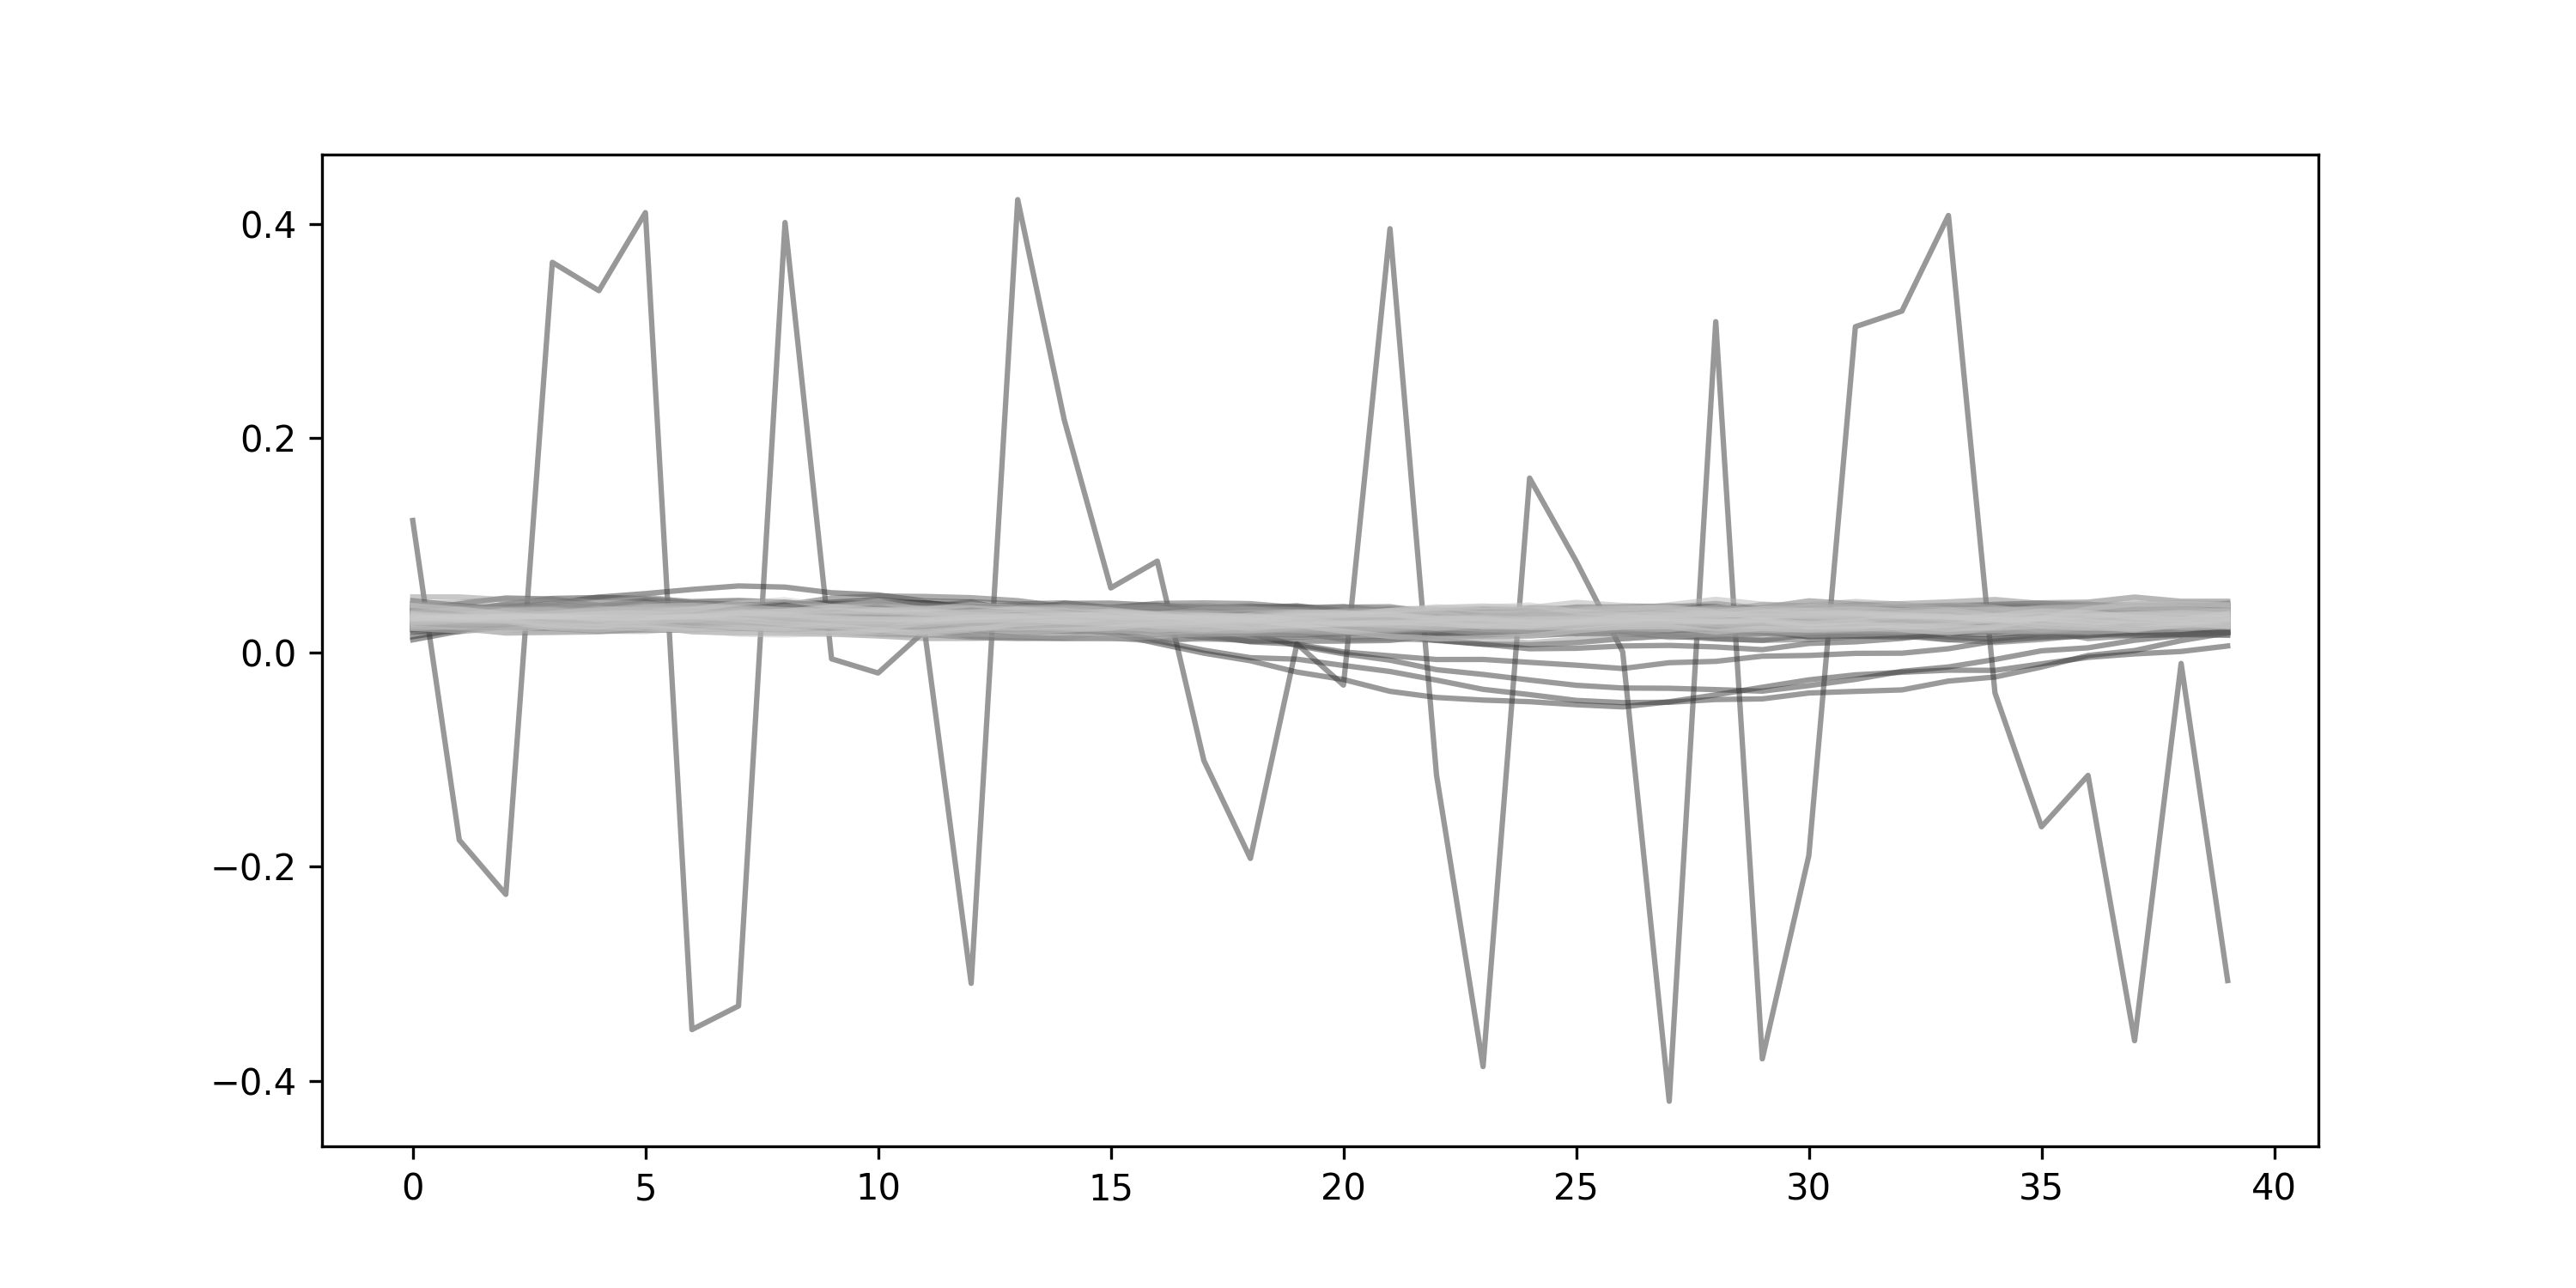
\includegraphics[width=0.3\textwidth]{../figs/math/long_range_experiment.png}
    & 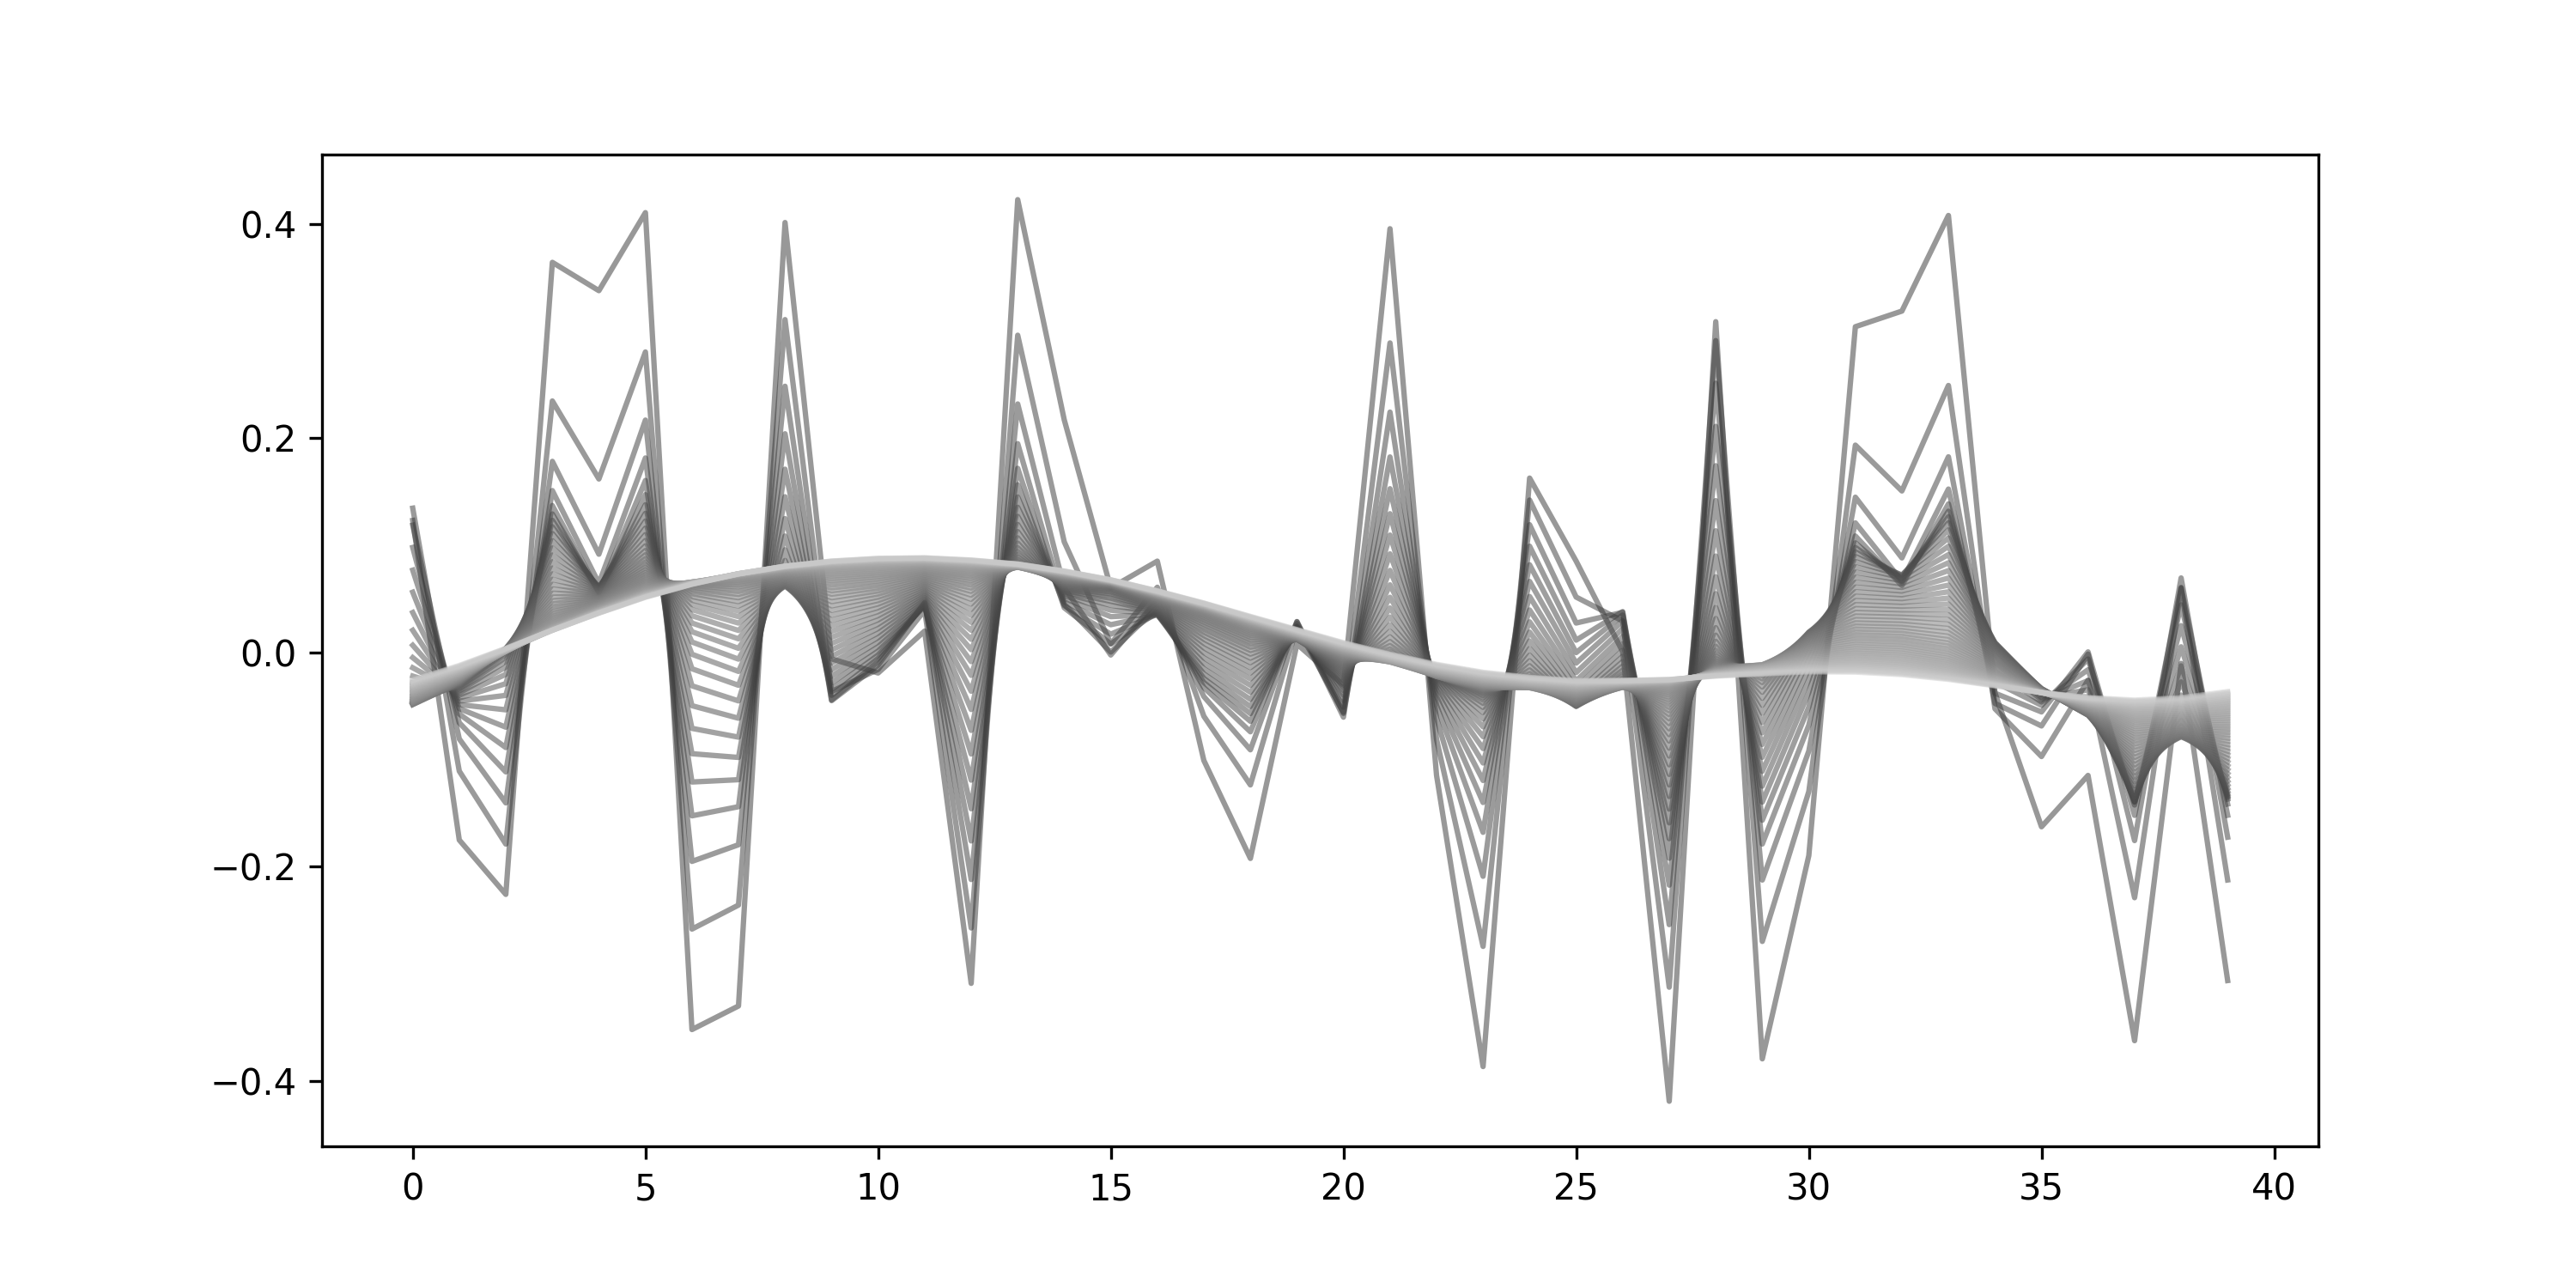
\includegraphics[width=0.3\textwidth]{../figs/math/long_range_theory.png}
    & 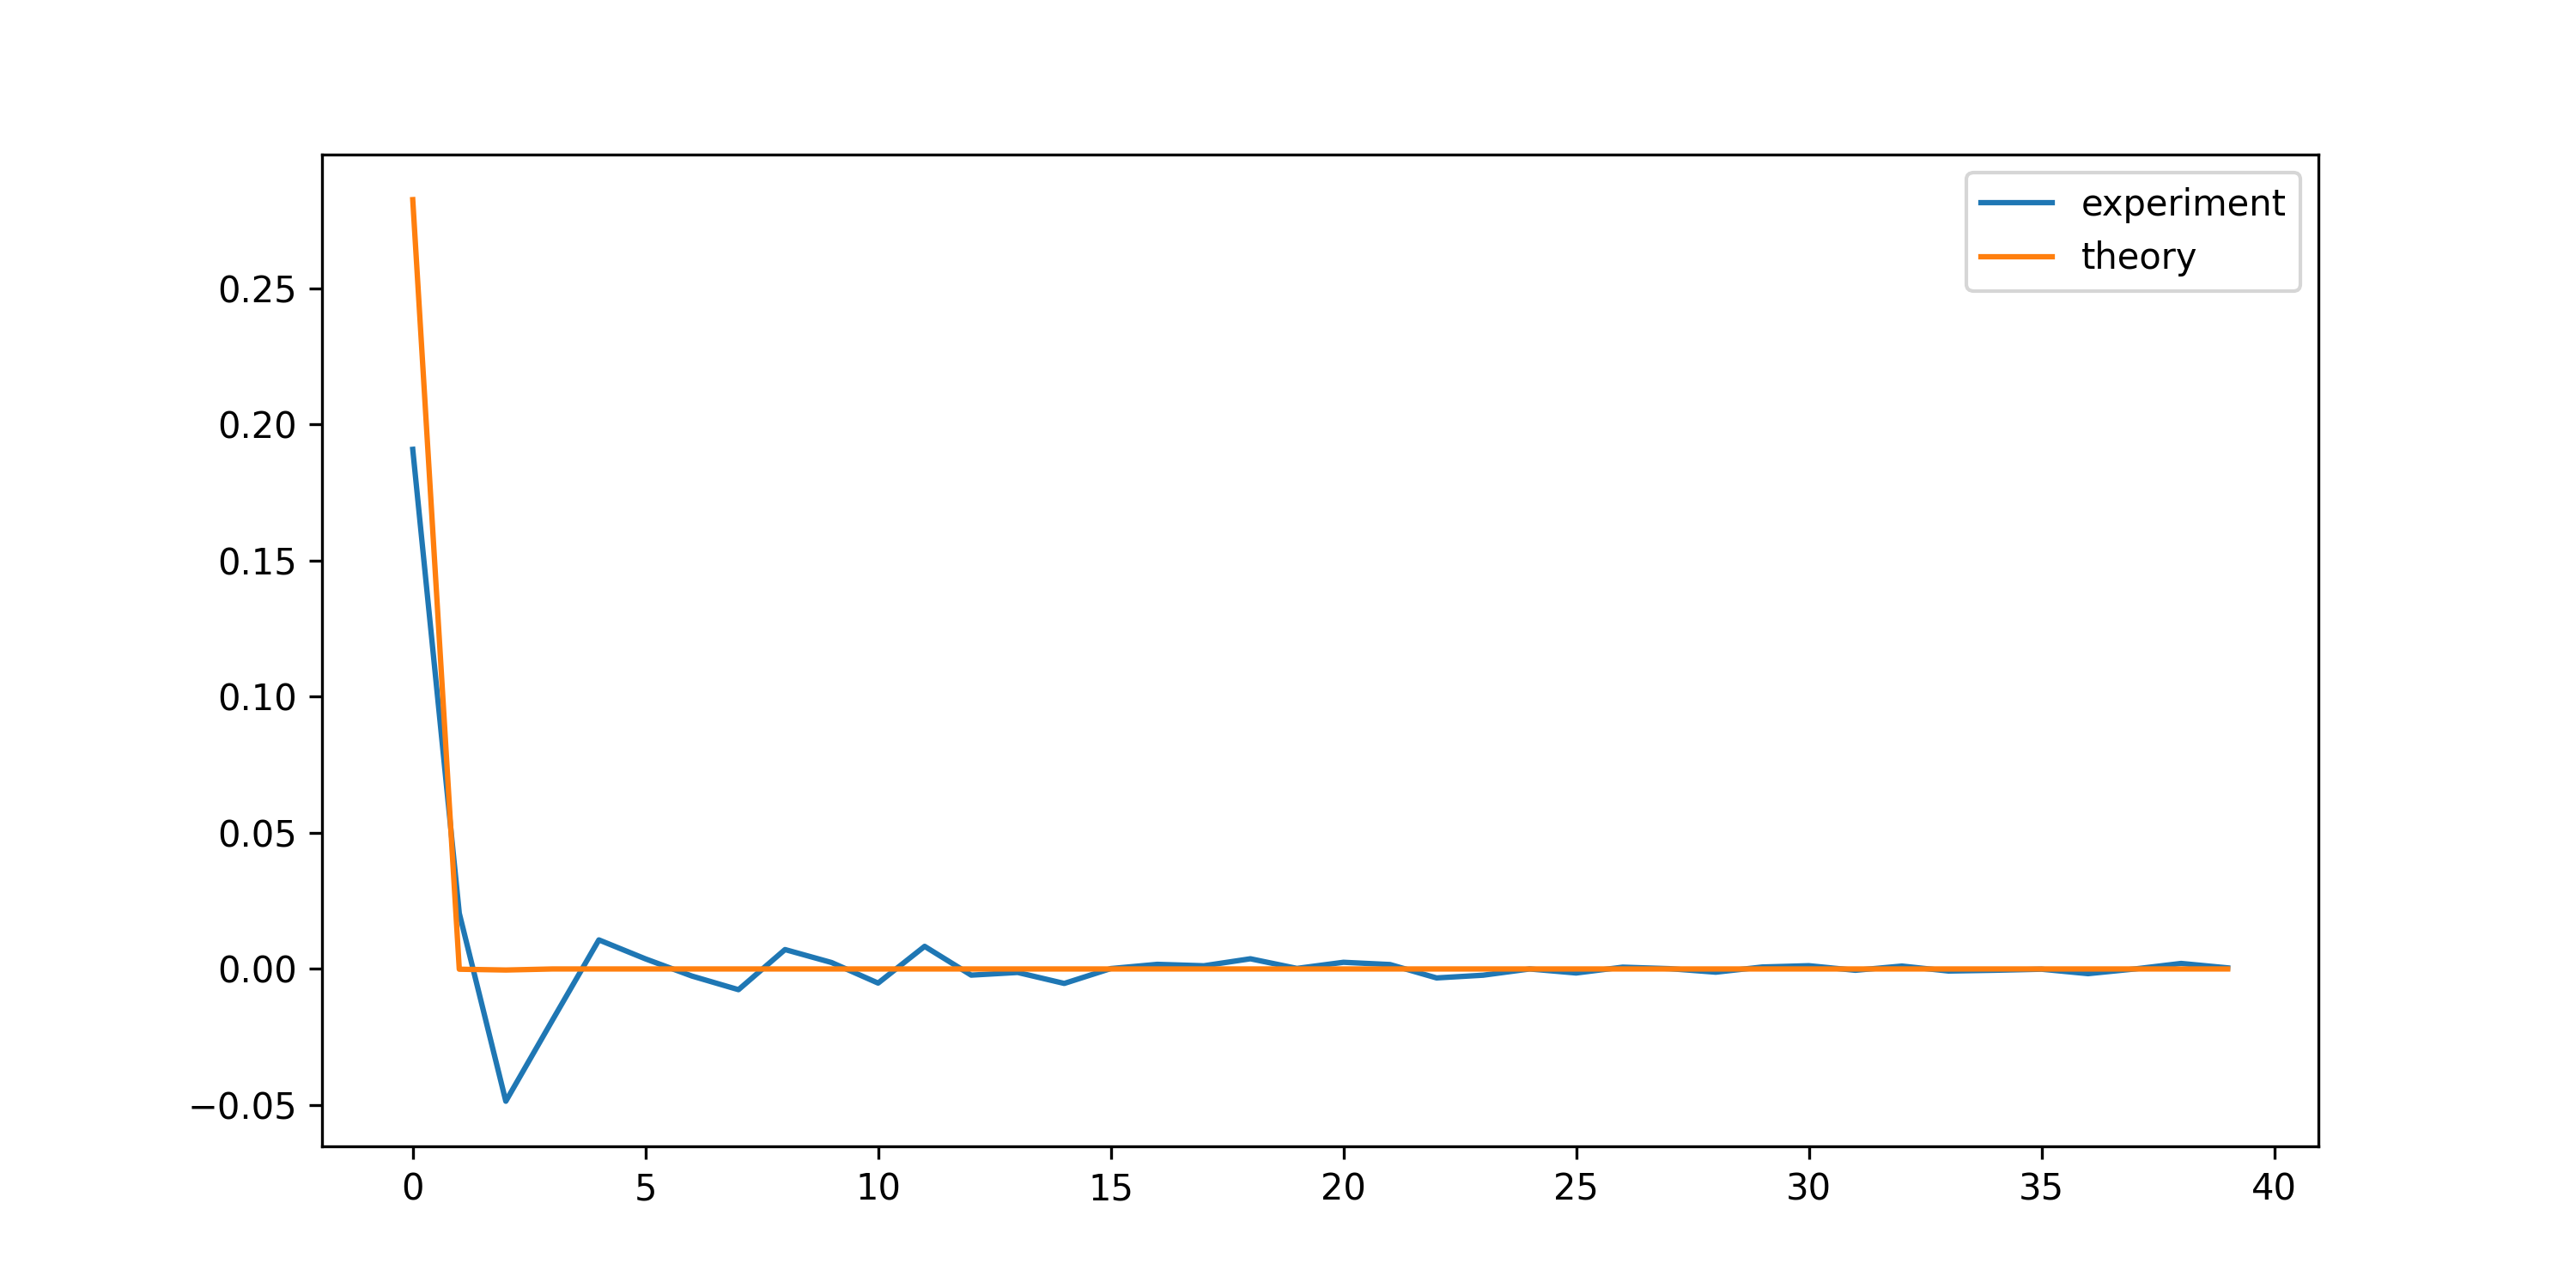
\includegraphics[width=0.3\textwidth]{../figs/math/theory_vs_experiment.png} \\
    (a) & (b) & (c)
  \end{tabular}
  \caption{
    Time-evolution of empirical (a) and theoretical (b) receptive fields for a single neuron with Gaussian data, along with (c) the final empirical vs. theoretical receptive fields in frequency space.
    Task settings: $\xi_1 = 2, \xi_2 = 1, g = 0.01, n = 40$.
    Training settings: learning rate of 0.01, batch size of 10,000, and 2,000 training steps with evaluations every 20.
    Model settings: $K=1$ with $w_1$ initialized from an Xavier normal with scale 1.
    }
  \label{fig:K1_receptive_fields}
\end{figure}

\paragraph*{Finding $u_1$}
We can't solve this ODE exactly, but we can try to find its steady state.
Write $\norm{u_1}_{\Lambda_1} = \sqrt{u_1^\top \Lambda_1 u_1}$.
Then, setting \cref{eq:grad_flow_K1_diag} to 0 yields
\begin{align}
  (\Lambda_0 + \Lambda_1) u_1 &= \sqrt{\frac{2}{\pi}} \frac{1}{\norm{u_1}_{\Lambda_1}} \Lambda_1 u_1.
\end{align}
We can look at this entrywise:
\begin{align}
  (\lambda_0^{(k)} + \lambda_1^{(k)}) u_1^{(k)} &= \sqrt{\frac{2}{\pi}} \frac{\lambda_1^{(k)}}{\norm{u_1}_{\Lambda_1}} u_1^{(k)}.
\end{align}
If $u_1^{(k)} \neq 0$, then
\begin{align}
  \frac{ \lambda_0^{(k)} }{ \lambda_1^{(k)} } + 1 &= \sqrt{\frac{2}{\pi}} \frac{1}{\norm{u_1}_{\Lambda_1}}.
\end{align}
So, in order for $u_1^{(k)}$ to be nonzero, we need the above equation to hold.
Note the right side is fixed for all $k$.
So we need $\frac{ \lambda_0^{(k)} }{ \lambda_1^{(k)} }$ to be constant for all $k$ such that $u_1^{(k)}$ is nonzero.

Recall we defined our eigenvectors to be the real and imaginary parts of the columns of the discrete Fourier transform, with the exception of the first and last eigenvectors.
So, eigenvalues will come in pairs, with the exception of the first and last eigenvalues.
Empirically, we observe that these pairs are all distinct.
So, only one or two of the eigenvectors will ever be nonzero.
If it is one, we will have
\begin{align}
  \frac{ \lambda_0^{(k)} }{ \lambda_1^{(k)} } + 1 &= \sqrt{\frac{2}{\pi}} \frac{1}{ (u_1^{(k)})^2 \lambda_1^{(k)} }
  % \iff
  % \lambda_0^{(k)} (u_1^{(k)})^2 + (u_1^{(k)})^2 \lambda_1^{(k)} = \sqrt{\frac{2}{\pi}}
  \iff
  (u_1^{(k)})^2 = \sqrt{ \frac{2}{\pi} } \frac{1}{ \lambda_0^{(k)} + \lambda_1^{(k)} }.
\end{align}

If it is two, we will see a superposition of the real and imaginary parts of the corresponding discrete Fourier transform column.
\begin{align}
  \frac{ \lambda_0^{(k_1)} }{ \lambda_1^{(k_1)} } + 1
  &= \frac{ \lambda_0^{(k_2)} }{ \lambda_1^{(k_2)} } + 1
  = \sqrt{\frac{2}{\pi}} \frac{1}{ (u_1^{(k_1)})^2 \lambda_1^{(k_1)} + (u_1^{(k_2)})^2 \lambda_1^{(k_2)} }
\end{align}
\begin{align}
  \sqrt{\frac{2}{\pi}} 
  &= \left( \frac{ \lambda_0^{(k_1)} }{ \lambda_1^{(k_1)} } + 1 \right) \left( (u_1^{(k_1)})^2 \lambda_1^{(k_1)} + (u_1^{(k_2)})^2 \lambda_1^{(k_2)} \right) \\
  &= \lambda_0^{(k_1)} (u_1^{(k_1)})^2 + \frac{ \lambda_0^{(k_1)} \lambda_1^{(k_2)} }{ \lambda_1^{(k_1)} } (u_1^{(k_2)})^2 + (u_1^{(k_1)})^2 \lambda_1^{(k_1)} + (u_1^{(k_2)})^2 \lambda_1^{(k_2)} \\
  &= \left[ \lambda_0^{(k_1)} + \lambda_1^{(k_1)} \right] (u_1^{(k_1)})^2 + \left[ \frac{ \lambda_0^{(k_1)} }{ \lambda_1^{(k_1)} } + 1 \right] \lambda_1^{(k_2)} (u_1^{(k_2)})^2.
\end{align}
Similarly,
\begin{align}
  \sqrt{\frac{2}{\pi}} 
  &= \left( \frac{ \lambda_0^{(k_2)} }{ \lambda_1^{(k_2)} } + 1 \right) \left( (u_1^{(k_1)})^2 \lambda_1^{(k_1)} + (u_1^{(k_2)})^2 \lambda_1^{(k_2)} \right) \\
  &= \left[ \frac{ \lambda_0^{(k_2)} }{ \lambda_1^{(k_2)} } + 1 \right] \lambda_1^{(k_1)} (u_1^{(k_1)})^2 + \left[ \lambda_0^{(k_2)} + \lambda_1^{(k_2)} \right] (u_1^{(k_2)})^2.
\end{align}
We could solve for $u_1^{(k_1)}$ and $u_1^{(k_2)}$ in terms of $\lambda_0^{(k_1)}, \lambda_1^{(k_1)}, \lambda_0^{(k_2)}, \lambda_1^{(k_2)}$.
But what's the point right now?

We still do not know which eigenvalues will be nonzero.
Empirically, in the \emph{very long limit}, it's only the first eigenvalue that is nonzero.
This corresponds to a flat receptive field.
Interestingly, for the data shown above, $k=1$ has the smallest ratio $\frac{ \lambda_0^{(k)} }{ \lambda_1^{(k)} }$ and the smallest inverse sum $\frac{ 1 }{ \lambda_0^{(k)} + \lambda_1^{(k)} }$.
I think this means its update is affected least by changes in $\norm{ u_1 }_{\Lambda_1}$.
I am not sure if this will generalize.

% This value is fixed for all $k$.
% Given that it's fixed, we want to work backwards and solve for $u_1^{(k)}$.
% Let $\KK$ be the set of indices $k$ for which $u_1^{(k)} \neq 0$.
% Then,
% \begin{align}
%   \sum_{l \in \KK } \lambda_1^{(l)} (u_1^{(l)})^2
%   &= \frac{2}{\pi} \frac{1}{(\lambda_0^{(k)} + \lambda_1^{(k)})^2} \qquad \forall k \in \KK. \label{eq:K1_u1_constraint}
% \end{align}
% When solving for $u_1$, $\Lambda_1$ and $\Lambda_0$ are fixed.
% So, we need to do a search over subsets \textit{and} over the nonzero entries of $u_1$.
% Clearly, for all $k \in \KK$, the right side of \cref{eq:K1_u1_constraint} must be the same.
% So, we can partition $[n]$ into disjoint sets $\KK_1, \dots, \KK_m$ such that for all $k,k' \in \KK_p$, $\lambda_0^{(k)} + \lambda_1^{(k)} = \lambda_0^{(k')} + \lambda_1^{(k')}$ (we can drop the $\pm$ because we know the eigenvalues are nonnegative).
% \emph{TODO: How do we proceed from here?}

\paragraph*{Conclusion}
Recall that we need to assume the data are Gaussian to conclude that $A X$ and $S$ are independent.
This is necessary to compute the conditional expectations.
One would hope that the general form remains the same for non-Gaussian data, but we cannot say anything precise.
One might assume that the case that the change in the distribution of the eigenvalues for $\Sigma_1$ and $\Sigma_0$ alone might account for this difference.
However, recall that the eigenvalues are derived from the covariance matrix, which is just a second-order statistic.
So, a Gaussian with the same covariance matrix would have the same eigenvalues.
However, Alessandro showed that if you train on Gaussian with covariance matching the non-Gaussian case, you do not get localization.
So, there is something other than just modifying $\Lambda_1$ and $\Lambda_0$ that changes the dynamics in \cref{eq:grad_flow_K1_diag} in the non-Gaussian case.

It is surprising that $w_1(t)$ pops out of the input-output term.
This \emph{does not happen in the gated linear network}, and this might be a key difference.
What does this say about gating early during training?
% I should double-check this to make sure it's right.
% If this weren't the case though, we would get a bias term that probably yields localization (or some nonzero structure).


\paragraph*{Fourier transforms}
Above, we just introduced the discrete Fourier transform matrix without explaining what it looks like.
Now, we'll quickly explain what it is and how we can simplify it when we have a real symmetric circulant matrix.

In a nutshell, circulant matrices diagonalize in the discrete Fourier basis because they act as convolutions on vectors.
This is clear from their definition:
\begin{align}
  \Sigma &= 
  \begin{bmatrix}
    c_0 & c_{n-1} & \cdots & c_2 & c_1 \\
    c_1 & c_0 & c_{n-1} &  & c_2 \\
    \vdots & c_1 & c_0 & \ddots & \vdots \\
    c_{n-2} &  & \ddots & \ddots & c_{n-1} \\
    c_{n-1} & c_{n-2} & \cdots & c_1 & c_0
  \end{bmatrix}.
\end{align}
It is easiest to understand the discrete Fourier transform matrix $P$ by seeing how its columns are constructed:
\begin{align}
  F_{:,j} 
  &= v_j
  \equiv \frac{1}{\sqrt{n}} \begin{bmatrix} 1 \\ \omega^j \\ \omega^{2j} \\ \vdots \\ \omega^{(n-1)j} \end{bmatrix}
  = \frac{1}{\sqrt{n}} \begin{bmatrix} 1 \\ \cos( \frac{2 \pi}{n} j ) \\ \cos( \frac{2 \pi}{n} 2j ) \\ \vdots \\ \cos( \frac{2 \pi}{n} (n-1) j ) \end{bmatrix}
  - \frac{i}{\sqrt{n}} \begin{bmatrix} 0 \\ \sin( \frac{2 \pi}{n} j ) \\ \sin( \frac{2 \pi}{n} 2j ) \\ \vdots \\ \sin( \frac{2 \pi}{n} (n-1) j ) \end{bmatrix},
\end{align}
where $\omega = e^{-\frac{2 \pi i}{n}}$.
So, each column is a sinusoid of an increasing frequency.
These columns are unit vectors and orthogonal to each other.
So, when we multiply a vector by $F$, we compute its coefficient w.r.t. to this basis.
This is analogous to computing the Fourier transform of a signal.

When our circulant matrix is real and symmetric ($c_i = c_{n-i}$ $\forall 1 \leq i < n$), we know from the spectral decomposition that we could diagonalize it using real eigenvectors.
Specifically, we can use the real and imaginary parts of the columns of $P$:
\begin{align}
  \Sigma (\re v_j)
  &= \re( \Sigma v_j )
  = \re( \lambda_j v_j )
  = \lambda_j (\re v_j),% \\
  % \Sigma (\im v_j)
  % &= \im( \Sigma v_j )
  % = \im( \lambda_j v_j )
  % = \lambda_j (\im v_j).
\end{align}
since the eigenvalues are real.
We can do the same for the imaginary parts.
Then, we just need to select the real and imaginary parts of the columns of $F$ to get a real orthogonal matrix.
Notice an immediate redundancy in the real parts:
\begin{align}
  \re v_j
  &= \frac{1}{\sqrt{n}} \begin{bmatrix} 1 \\ \cos( \frac{2 \pi}{n} j ) \\ \cos( \frac{2 \pi}{n} 2j ) \\ \vdots \\ \cos( \frac{2 \pi}{n} (n-1) j ) \end{bmatrix}
  = \frac{1}{\sqrt{n}} \begin{bmatrix} 1 \\ \cos( \frac{2 \pi}{n} (n-1)j ) \\ \cos( \frac{2 \pi}{n} (n-2)j ) \\ \vdots \\ \cos( \frac{2 \pi}{n} j ) \end{bmatrix}
  = \re v_{n-j}.
\end{align}
So, we only need to consider the real parts of first $\frac{n}{2}$ columns of $F$.
The same can be said for the imaginary parts, though we ignore the first column since it is all zeros, and take the $\frac{n}{2}+1$-th real column in its place.
If we sort the columns by frequency, we get the sinusoids shown in \cref{fig:fourier_transform_matrix}.
\begin{figure}
  \centering
  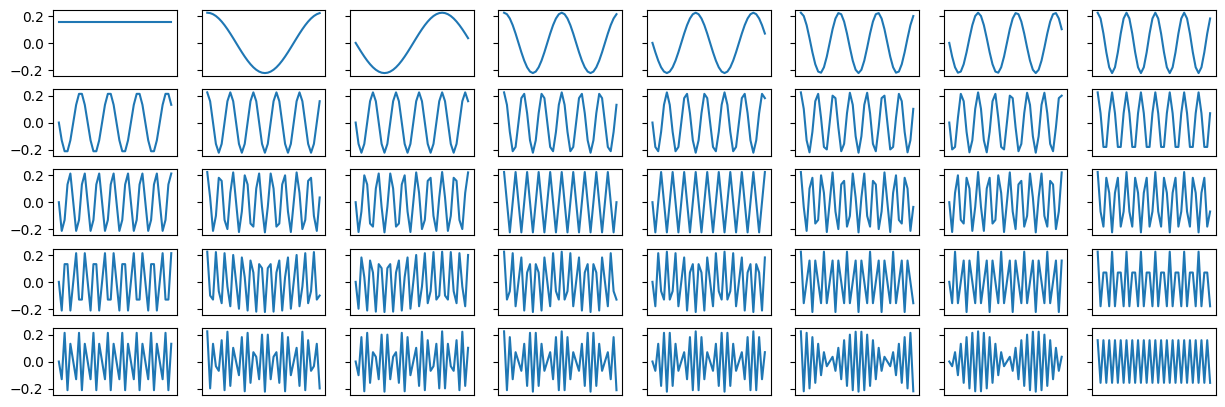
\includegraphics[width=0.8\textwidth]{../figs/math/fourier_transform_matrix.png}
  \caption{Discrete sine/cosine transform matrix $F$ for $n=40$.}
  \label{fig:fourier_transform_matrix}
\end{figure}


%%%%%%%%%%%%%%%%%%%%%%%
%% Non-Gaussian Data %%
\subsection*{Non-Gaussian Data}
We needed Gaussianity to say that $A X$ and $S$ were independent.
Our construction of $v$ and $A$ was chosen to make $A X$ and $S$ have zero covariance.
For general data, this does not imply independence.
So, we will have to do something else to compute the conditional expectations.

What do we know about $X$?
First, it is symmetric about 0, and it is translation invariant.
As $g \to \infty$, $X_i(Z) \overset{d}{\to} \text{sign}(Z_i)$.
Deriving the pmf of $X$ in this limit amounts to solving the ``orthant problem'' for multivariate normals.
For inputs of dimension larger than 4, this is an open research problem.
So, I don't think we'll have much luck here.
For what it's worth, we don't need full information about the distribution, just the conditional expectations.
But I struggle to see how we could compute this if we cannot even compute the pmf.

\paragraph*{Basis initialization}
What if we initialize the weights to be the basis vectors for $\R^n$?
(This is the same as the ``small bump'' gate we show below.)
I am going to break the law and cite that result here without showing any work.
For $X \triangleq \operatorname{erf}(g Z)$,
\begin{align}
  \E_{ X, \langle X, e_i \rangle > 0 \mid Y = 1 } \left[ \langle X, e_i \rangle \right] 
\end{align}


%%%%%%%%%%%%%%%%%%%%%%%%%%%%%%%%%%%%%%
%% Have You Tried Making It Linear? %%
%%%%%%%%%%%%%%%%%%%%%%%%%%%%%%%%%%%%%%
\section{Have You Tried Making It Linear?}

% \emph{When in doubt, take the nonlinearities out!}
Gating lets us decompose the ReLU post-activation in terms of the pre-activation's sign and magnitude.
\begin{align}
  \text{ReLU}(\langle w_1(t), x \rangle)
  &= g(t, x) \langle w_1(t), x \rangle \qquad \text{where} \qquad g(t, x) = \mathbbm{1}( \langle w_1(t), x \rangle \geq 0 ). \label{eq:relu_gating}
\end{align}
We generally assume that $g$ does not vary during learning, even though $w_1$ may.
Later on, we'll try to analyze what happens when this does not hold.

To assess the validity of this assumption, we need to see how much $g(x)$, as defined above, changes during learning.
Additionally, post-hoc, we can usually pick a somewhat sensible gating structure that mimics a specific run's behavior.
But we'd like to be able to determine this gating upfront.
We explore all this in the following subsections.

\subsection{Sign Flipping}

We will model the ReLU network as in \cref{eq:relu_gating}, focusing on how $g$ varies with time for each hidden neuron.
We will look at the metric%s
\begin{align}
  p(t) &= \PR_x( g(t, x) = g(t + \delta t, x) ) \qquad \text{for all $t$}.% \\
  % p_{\text{unif}} &= \PR_x( \{ g(t, x) = g(t', x) \ \forall t,t' \} )
\end{align}

Note that $g$ is invariant to the scale of $w_1$.
We observe in the experiments above that $w_1$ appears to grow uniformly in size during much of its training, appearing as if it's just being scaled up towards its final value.
If this isn't true in position space, it seems more likely to be true in frequency space, though it only seems to really hold in the long-range oscillation case.
This is probably not a very good assumption during the early stage of training, but it seems more plausible once they have stabilized a bit.
There is, importantly, a phase where the receptive field goes from Gaussian to non-Gaussian, but the shape it assumes at the end of training emerges quite quickly.
This suggests that $g(x)$ may be relatively constant during learning, at least after the initial phase.
If this is so, then it would be reasonable to try using a standard GDLN to model the ReLU network.

This is precisely what we check in \cref{fig:sign_flipping}.
We see that at any given time, gates, on average, flip sign for a very small fraction of the data, and this happens less as training progresses.
However, the fact that there is still some sign flipping means we cannot—with confidence—naively apply a GDLN to model the ReLU network.
We will try this next, but it's not obvious what the gates should be a prirori, which lead us to questions about how to interpret the neural race.

\begin{figure}
  \centering
  \includegraphics[width=0.8\textwidth]{{"../figs/sign_flipping/NonlinearGPDataset_40_12_2_1_0.01_1.0_lr0.01"}.png}
  \caption{
    Sign flipping in the NLGP dataset.
    Blue shows $p(t)$ across $t$.
    Green shows excess kurtosis of preactivations to a single neuron.
    Red shows the final receptive fields for the corresponding neuron.
    Task settings: $\xi_1 = 2, \xi_2 = 1, g = 0.01, n = 40$.
    Training settings: learning rate of 0.01, batch size of 10,000, and 5,000 training steps with evaluations every 20.
    Model settings: $K=12$ with weights initialized from an Xavier normal with scale 1.
  }
  \label{fig:sign_flipping}
\end{figure}


\subsection{Predicting Loca(liza)tion}
TODO: can we predict where localization will occur a priori?

% \subsection{Evolving Gates?}


%%%%%%%%%%%%%%%%%%%%%%%%%%%%%%%%%%%%%%%%%%%%%%%%%%%%%%%%%%%%%
%% Let's Consider a Single Layer with Linear Activation... %%
%%%%%%%%%%%%%%%%%%%%%%%%%%%%%%%%%%%%%%%%%%%%%%%%%%%%%%%%%%%%%
\section{Let's Consider a Single Layer with Linear Activation...}

Our GDLN model is defined as follows:
\begin{align}
  \hat{y}(x) &= \frac{1}{K} \left( \sum_{k \in [K]} g_k(x) w_k^\top \right) x, \label{eq:gdln_model}
\end{align}
where $g_k$ are (node) gates.
Again, $w_k \in \R^n$ are the rows of the first-layer weight matrix $W_1 \in \R^{K \times n}$.
That is,
\begin{align}
  W_1 &= \begin{pmatrix} w_1^\top \\ \vdots \\ w_K^\top \end{pmatrix}
\end{align}

Recalling the GDLN paper, the gradient flow for $w_1$ is given by
\begin{align}
  \tau \frac{d}{dt} w_1 &= \frac{1}{K} \left[ \Sigma^{yx}(p_1) - \sum_{k \in [K]} \Sigma^{xx}(p_1,p_k) w_k \right], \label{eq:grad_flow}
\end{align}
where
\begin{align}
  \Sigma^{yx}(p_i) &= \E_{g,X,Y} \left[ g_i Y X \right] \\
  \Sigma^{xx}(p_i,p_j) &= \E_{g,X,Y} \left[ g_i g_j X X^\top \right].
\end{align}

All rows $w_k$ of $W_1$ have gradient flows of this form.
Let us analyze them all simultaneously.
To do so, let us relabel $b_i = \Sigma^{yx}(p_i)$ and $A_{ij} = \Sigma^{xx}(p_i,p_j)$.
Note that $A_{ij}$ is symmetric and $A_{ij} = A_{ji}$.
Then, we can write the gradient flow for all weights as
\begin{align}
  K \tau \frac{d}{dt} \underbrace{\begin{bmatrix} w_1 \\ \vdots \\ w_K \end{bmatrix}}_{w \in \R^{Kn}}
  &= \underbrace{\begin{bmatrix} b_1 \\ \vdots \\ b_k \end{bmatrix}}_{b \in \R^{Kn}} - \underbrace{\begin{bmatrix} A_{11} & \cdots & A_{1K} \\ \vdots & \ddots & \vdots \\ A_{K1} & \cdots & A_{KK} \end{bmatrix}}_{A \in \R^{Kn \times Kn}} \begin{bmatrix} w_1 \\ \vdots \\ w_K \end{bmatrix}. \label{eq:grad_flow_matrix}
\end{align}
Observe that $w$ is the vectorized form of our $K \times n$ first-layer weight matrix.
Note also that $A$ is a symmetric real matrix, so we can diagonalize it as $A = P \Lambda P^\top$, where the columns of $P$ are the eigenvectors of $A$ and the diagonal entries of $\Lambda$ are the corresponding (nonnegative) eigenvalues.
% (It is symmetric because $A$ is block symmetric with blocks $A_{ij}$, and the blocks are also symmetric.)
To see this more clearly, let us write
\begin{align}
  \tilde{g}(x) &= \begin{bmatrix} g_1(x) \\ \vdots \\ g_K(x) \end{bmatrix}. % \in \{ 0,1 \}^K.
\end{align}
Then,
\begin{align}
  A &= \left\langle (\tilde{g} \otimes X) (\tilde{g} \otimes X)^\top \right\rangle_{g,X}, \label{eq:A_kron}
\end{align}
which is clearly a symmetric matrix.
% (Interjection: Whatever distribution we have over $g$ should satisfy that $\tilde{g} \sim \Pi \tilde{g}$, where $\Pi$ is some permutation matrix on $K$ elements.
% That is, the distribution should be invariant to the ordering of the gates, since this is what we want empirically.
% So, for a finite dataset with $|X|$ elements and binary gates, there are $\frac{2^{K |X|}}{K !}$ unique gating architectures, up to permutation.
% FIXME: this can't be true...
% )

We can reparameterize in terms of $u = P^\top w$ and $c = P^\top b$.
\begin{align}
  K \tau \frac{d}{dt} u &= - \Lambda u + c
  \implies
  u(t) = \Lambda^{-1} e^{ -\frac{t}{K \tau} \Lambda + C } \mathbf{1} + \Lambda^{-1} c,
\end{align}
where $C$ is a constant diagonal matrix that defines the initial condition.
So,
\begin{align}
  w(t) 
  &= P \Lambda^{-1} e^{ -\frac{t}{K \tau} \Lambda + C } \mathbf{1} + P \Lambda^{-1} c \\
  &= A^{-1} P e^{ -\frac{t}{K \tau} \Lambda + C } \mathbf{1} + A^{-1} b. \label{eq:grad_flow_solution}
\end{align}


%% Exclusive gates %%
\paragraph*{Exclusive Gates}
Let us assume that the gates are exclusive, that is, only one gate is active at a time.
Then, $\Sigma^{xx}(p,q) = 0$ for $p \neq q$, which makes $A$ block diagonal.
We can write the gradient flow for $w_1$ as
\begin{align}
  K \tau \frac{d}{dt} w_1 &= - A_{11} w_1 + b_1.
\end{align}
Note that $A_{11} = \Sigma^{xx}(p_1, p_1)$ is always symmetric (and real).
So, we can diagonalize it to solve the ODE.
If we do this, we get
\begin{align} \label{eq:exclusive_gates_limiting_solution}
  w_1(\infty) &= ( \Sigma^{xx}(p_1,p_1) )^{-1} \left( P e^{ -\frac{t}{\tau} \Lambda + C } \mathbf{1} + \Sigma^{yx}(p_1)^\top \right),
\end{align}
where $C$ is some constant diagonal matrix that defines the initial condition.
As with above, this is the population solution to OLS, $( \E_{X,Y} \left[ X X^\top \right] )^{-1} \E_{X,Y} \left[ Y X \right]$.
% $(X^\top X)^{-1} X^\top y = ( \langle x x^\top \rangle )^{-1} ( \langle x y \rangle )$.
So, each weight matrix converges to the OLS solution on the subset of the data determined by its gate.


%%%%%%%%%%%%%%%%%%%%%%%%%%%%%%
%% Winning Gating Structure %%
\subsection{Winning Gating Structure}

Can we read off the winning gating structure from the equations above?
This is where we are unsure of how exactly to interpret the ``neural race.''
Is the idea that the gating structure that learns fastest in the GDLN is the one the ReLU network ends up implementing?
Or, is the idea to do some meta-optimization over gating structures to minimize the limiting loss of the corresponding GDLN, and propose that this is what ReLU somehow ``knows'' to use?
Are both perspectives insightful or meaningful?

We would answer the former by looking at the induced eigenvalues of $A$.
The ``race winner'' would be that which yields the smallest eigenvalues.
We would answer the latter by looking at the limiting loss of the GDLN.
The winner would be that which yields the smallest loss in the limit.
Both of these seem like complicated, though certainly empirically investigable, problems (though, the space of gates to search over is combinatorially large, if not infinite!).
We empirically analyze a few gating structures below.

%% Early Dynamics %%
\subsubsection{Do We Care About Early Dynamics?}
We wish to see which gating structures yield solutions with the smallest eigenvalues, since they will decay the slowest.
\hl{However, we have many eigenvalues, so which ones do we look at?}

For small $t$, but sufficiently large to see separation among different eigenvalues, can we predict the leading structure?

TODO: look into eigenvalues for some gating structures!
(Pick random, zero, and localized, for example.)

%% Limiting Behavior %%
\subsubsection{Or Limiting Behavior?}
If none of the eigenvalues are zero, then $w(\infty) = A^{-1} b$.
If we write
\begin{align}
  \tilde{x} &= \begin{bmatrix} g_1(x) x \\ \vdots \\ g_K(x) x \end{bmatrix} \in \R^{Kn},
\end{align}
then $A = \E_{g,X,Y} \left[ \tilde{X} \tilde{X}^\top \right]$ and $b = \E_{g,X,Y} \left[ Y \tilde{X} \right]$.
Then, it is clear that this is the population solution to the OLS problem of regressing $Y$ on $\tilde{X}$, averaging across the distributions of the data \textit{subject to} the gating architecture.

In this context, one might ask, which gating structure minimizes the MSE loss?
The loss is (note we use $\langle \rangle$ notation for brevity):
\begin{align}
  \LL_{\infty}
  &= \left\langle \left( \tilde{X}'^\top (\langle \tilde{X} \tilde{X}^\top \rangle_{g,X,Y})^{-1} \langle Y \tilde{X} \rangle_{g,X,Y} - Y' \right)^2 \right\rangle_{g',X',Y'}  \\
  &= \left\langle ( \tilde{X}'^\top (\langle \tilde{X} \tilde{X}^\top \rangle_{g,X,Y})^{-1} \langle Y \tilde{X} \rangle_{g,X,Y} )^2 - 2 ( Y' \tilde{X}'^\top (\langle \tilde{X} \tilde{X}^\top \rangle_{g,X,Y})^{-1} \langle Y \tilde{X} \rangle_{g,X,Y} ) + (Y')^2 \right\rangle_{g',X',Y'} \\
  &= \frac{1}{2} - \langle Y \tilde{X}^\top \rangle_{g,X,Y} (\langle \tilde{X} \tilde{X}^\top \rangle_{g,X,Y})^{-1} \langle Y \tilde{X} \rangle_{g,X,Y} \\
  &= \frac{1}{2} - \frac{1}{2} \langle \tilde{X} \rangle_{g, X \mid Y=1}^\top (\langle \tilde{X} \tilde{X}^\top \rangle_{g, X \mid y=1} + \langle \tilde{X} \tilde{X}^\top \rangle_{g, X \mid Y=0})^{-1} \langle \tilde{X} \rangle_{g, X \mid Y=1}. \label{eq:ols_loss}
\end{align}
% In the final step, we assumed (WLOG) that the negative class is $y=0$ and the positive class is $y=1$.
% (Throughout, we also assume that the classes are balanced.)
The ``meta-optimization'' question is: For fixed $p_{\xi_1}$ and $p_{\xi_2}$, how do we choose the gates $g_k$ to minimize \cref{eq:ols_loss}?

It may be useful to write this in terms of Kronecker products.
Let
\begin{align}
  \tilde{g}(x) &= \begin{bmatrix} g_1(x) \\ \vdots \\ g_K(x) \end{bmatrix} \in \{ 0,1 \}^K.
\end{align}
Then, minimizing \cref{eq:ols_loss} is equivalent to maximizing
\begin{align}
  \LL_{\infty}^*(\tilde{g}) &= \langle \tilde{g} \otimes X \rangle_{g, X \mid Y=1}^\top (\langle ( \tilde{g} \otimes X ) ( \tilde{g} \otimes X )^\top \rangle_{g, X \mid Y=1} + \langle ( \tilde{g} \otimes X ) ( \tilde{g} \otimes X )^\top \rangle_{g, X \mid Y=0})^{-1} \langle \tilde{g} \otimes X \rangle_{g, X \mid Y=1} \label{eq:ols_kron}
\end{align}
over $\tilde{g} : \supp(p_{\xi_1}) \cup \supp(p_{\xi_2}) \to \{0,1\}^K$.


%%%%%%%%%%%%%%%%%%%%%%%%%%%%%%%%%%%%
%% Structure in Limiting Behavior %%
\subsection{Structure in Limiting Behavior}
The limiting solution in \cref{eq:exclusive_gates_limiting_solution} assumes, of course, that the gates are fixed throughout training.
As we observe in \cref{fig:sign_flipping}, the gates stabilize relatively early on.
Our ReLU analysis was able to fully explain the behavior of a single neuron if we train with Gaussian data.
With the GDLN, if we know what the gate, $g(x)$, stabilizes to, then we can use the limiting solution to fully characterize the final receptive fields for both Gaussian \emph{and} non-Gaussian data.

Let us consider a gate of the form $g(x) = \mathbbm{1}( \langle e_i, x \rangle > 0)$.
This gate is turned on only when the $i$-th coordinate of $x$ is positive.
This is a simple case of a localized bump (and much easier to analyze).
We'll show that it explains the localization behavior we've observed in the converged weights of the ReLU network.

\paragraph*{Input-output covariance}
The interesting structure is in the input-output covariance.
Let's compute it.
\begin{align}
  \Sigma^{yx}(p_i) 
  &= \E_{g,X,Y} \left[ g_i Y X \right] \\
  &= \E_{X, \langle e_i, X \rangle > 0 \mid Y=1} \left[ X \right] \PR( Y=1 ) \\
  &= \E_{ Z_i > 0 } \left[ \E_{ Z \mid Z_i, Y=1 } \left[ \frac{ \operatorname{erf}( g Z ) }{ \mathcal{Z}(g) } \right] \right] \PR( Y=1 ).
\end{align}
In the final step, we use the fact that $X_i > 0 \iff Z_i > 0$.
This is not true if we take an inner product with something other than $e_i$—\emph{this is a big part of what makes the nonlinear case so hard to analyze}.
Here, $\mathcal{Z}(g)$ is the normalization constant that ensures the variance of each coordinate is 1 for all $g > 0$, which here represents the gain.
(Sorry about overloading notation here! In the GDLN work, $g$ is the gate, but in Alessandro's work it is the gain.
I didn't want to switch existing notation too much, and I think it's clear from context which one we mean.)

Let us evaluate the inner expectation.
We will suppress the conditioning on $Y=1$ for brevity.
Note that for $j \neq i$, $Z_j \mid Z_i \sim \NN\left( r Z_i, 1 - r^2 \right)$, where $r$ is the covariance between $Z_i$ and $Z_j$, which is equal to $e^{-(i-j)^2/\xi_1^2}$.
Thus,
\begin{align}
  \E_{Z \mid Z_i, Y=1} \left[ \operatorname{erf}(g Z_j) \right]
  &= \int_{\R} \operatorname{erf}(g z_j) \frac{1}{\sqrt{2 \pi \sqrt{1 - r^2}}} \exp\left( -\frac{(z_j - r z_i)^2}{2 (1 - r^2)} \right) dz_j \\
  &= \operatorname{erf}\left( \frac{ g r }{ \sqrt{ 1 + 2 g^2 (1-r^2) } } z_i \right).
\end{align}
Now, we can compute the outer expectation.
\begin{align}
  \E_{ Z_i > 0 } \left[ \E_{ Z \mid Z_i, Y=1 } \left[ \operatorname{erf}( g Z_j ) \right] \right]
  &= \int_0^\infty \frac{1}{\sqrt{2 \pi}} \exp\left( -\frac{z_i^2}{2} \right) \operatorname{erf}\left( \frac{ g r }{ \sqrt{ 1 + 2 g^2 (1-r^2) } } z_i \right) dz_i \\
  &= \frac{2}{\sqrt{\pi}} \tan^{-1} \left( \frac{ \sqrt{2} g r }{ \sqrt{ 1 + 2 g^2 (1-r^2) } } \right) \\
  &= \frac{2}{\sqrt{\pi}} \tan^{-1} \left( \frac{ r }{ \sqrt{ \frac{1}{2g^2} + (1-r^2) } } \right).
\end{align}
In summary,
\begin{align}
  \Sigma^{yx}(p_i)_j
  &= \frac{1}{\sqrt{\pi} \mathcal{Z}(g)} \tan^{-1} \left( \frac{ r }{ \sqrt{ \frac{1}{2g^2} + (1-r^2) } } \right).
\end{align}
Visualizing this in \cref{fig:sigma_yx}, we see that it produces a localized bump centered at $i$.
\begin{figure}
  \centering
  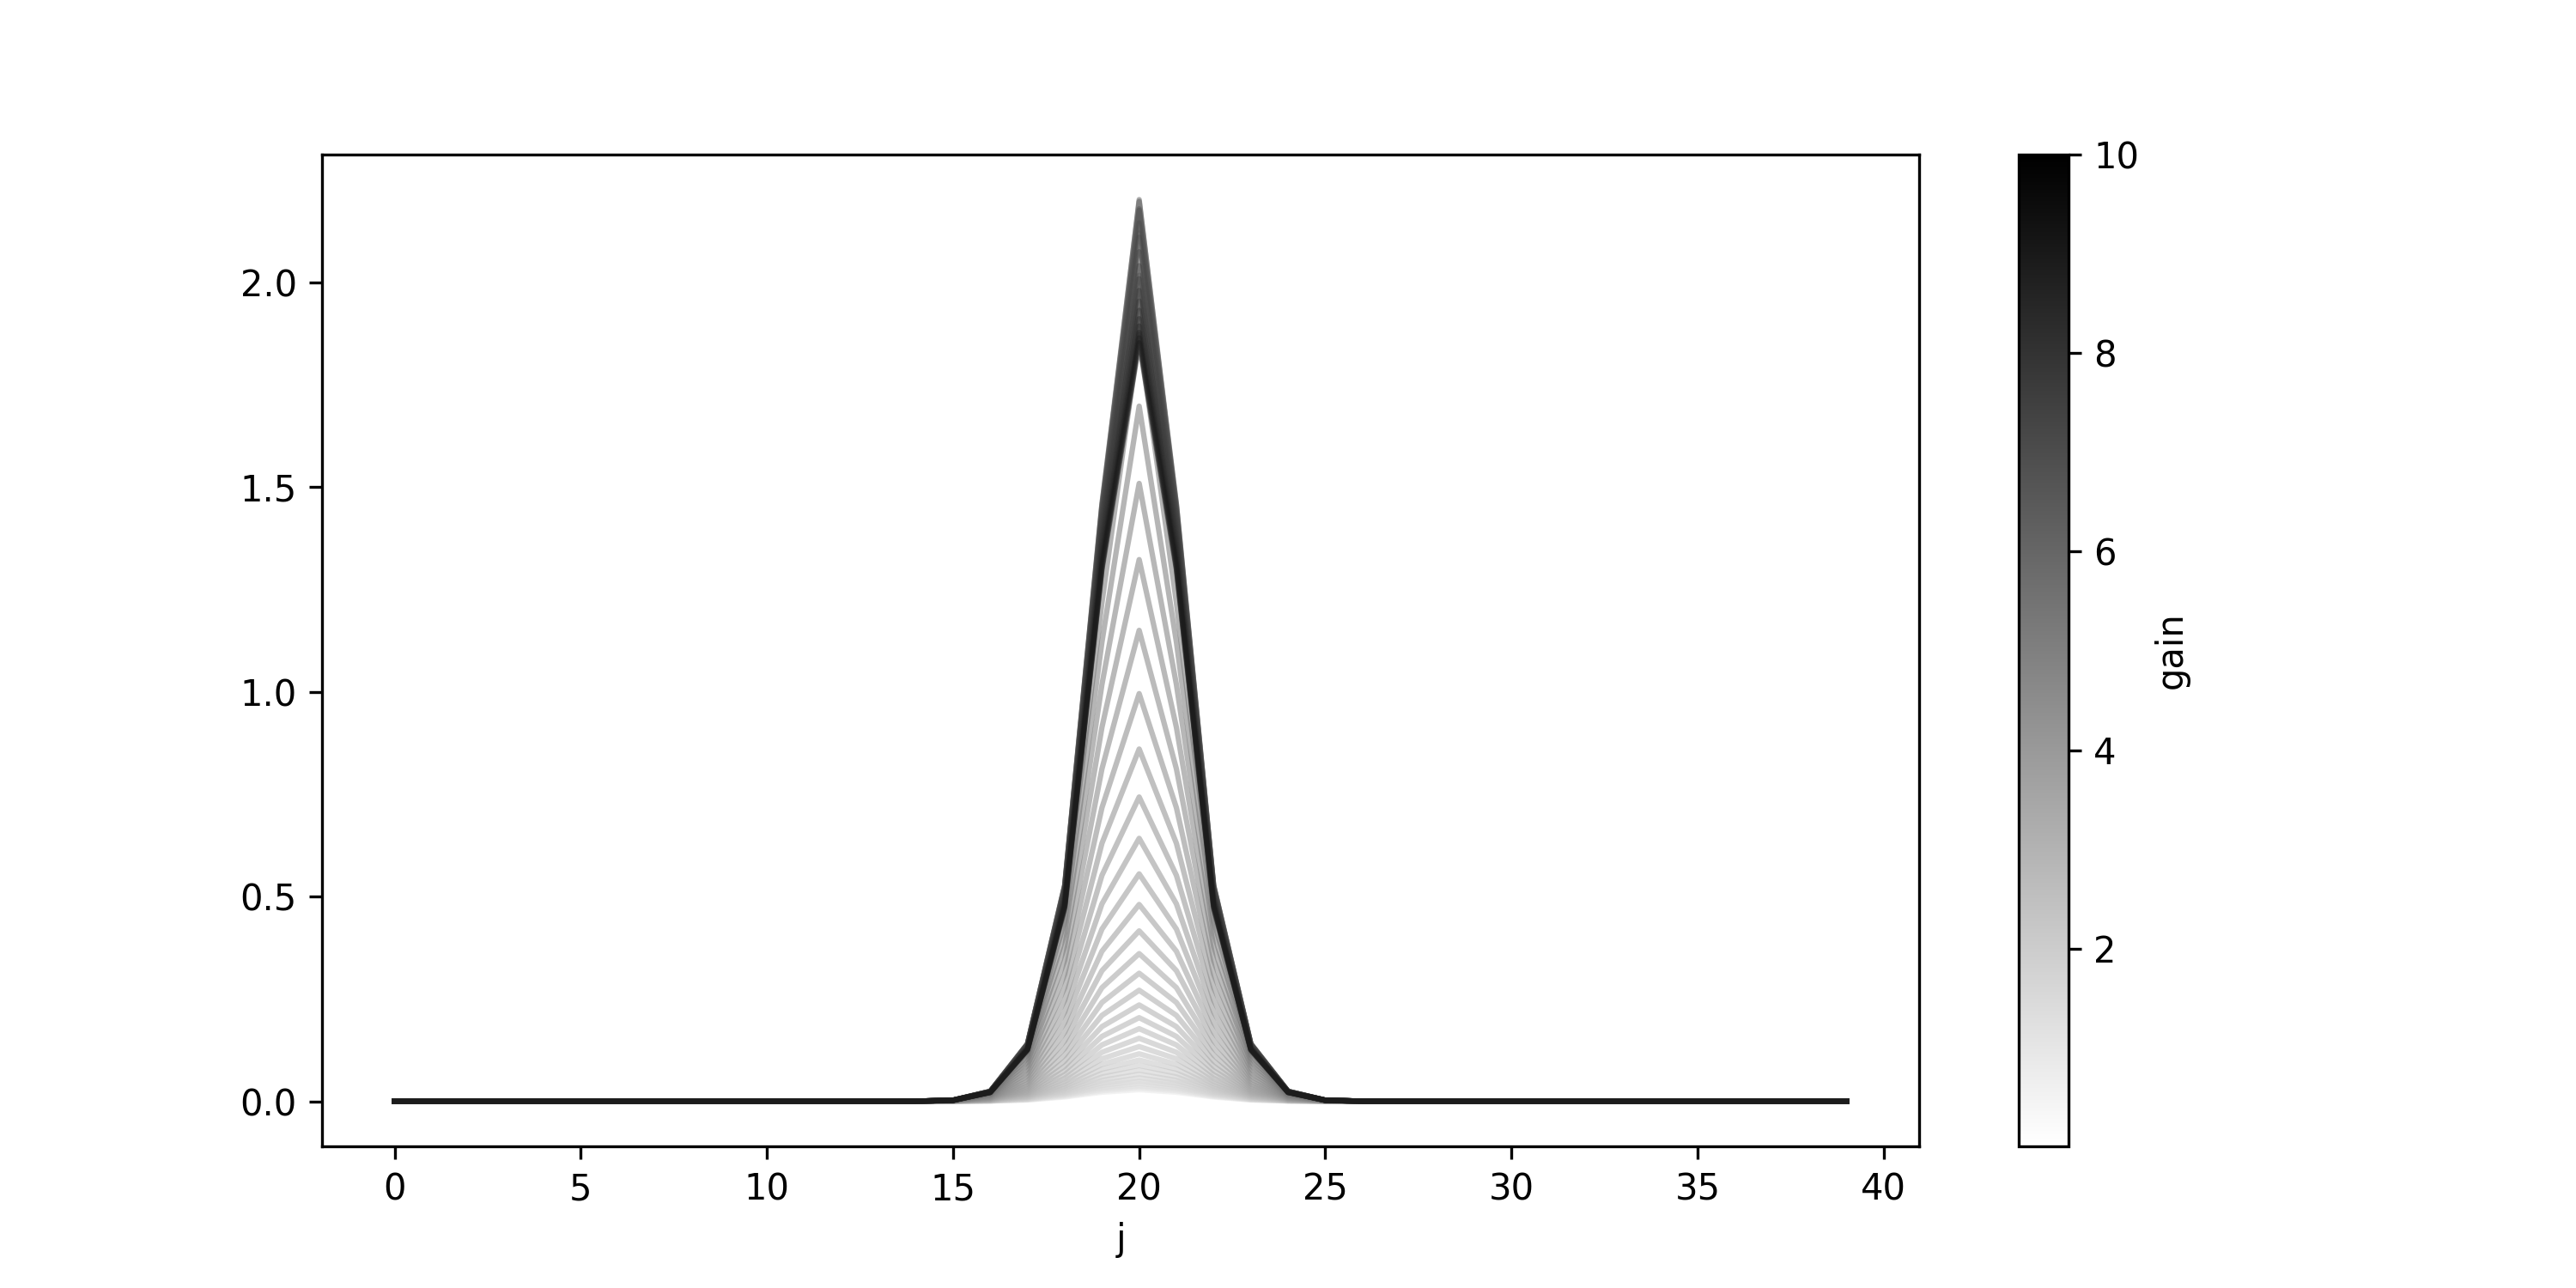
\includegraphics[width=0.8\textwidth]{../figs/math/sigma_yx.png}
  \caption{Entries $j$ of input-output covariance $\Sigma^{yx}(p_i)$ for $i=20$ for varying $g$.}
  \label{fig:sigma_yx}
\end{figure}
This is cool!
But what does the input-input covariance term do?
Well, for this gate, it basically computes a difference between adjacent points of $\Sigma^{yx}(p_i)$.
\begin{figure}
  \centering
  \begin{tabular}{cc}
    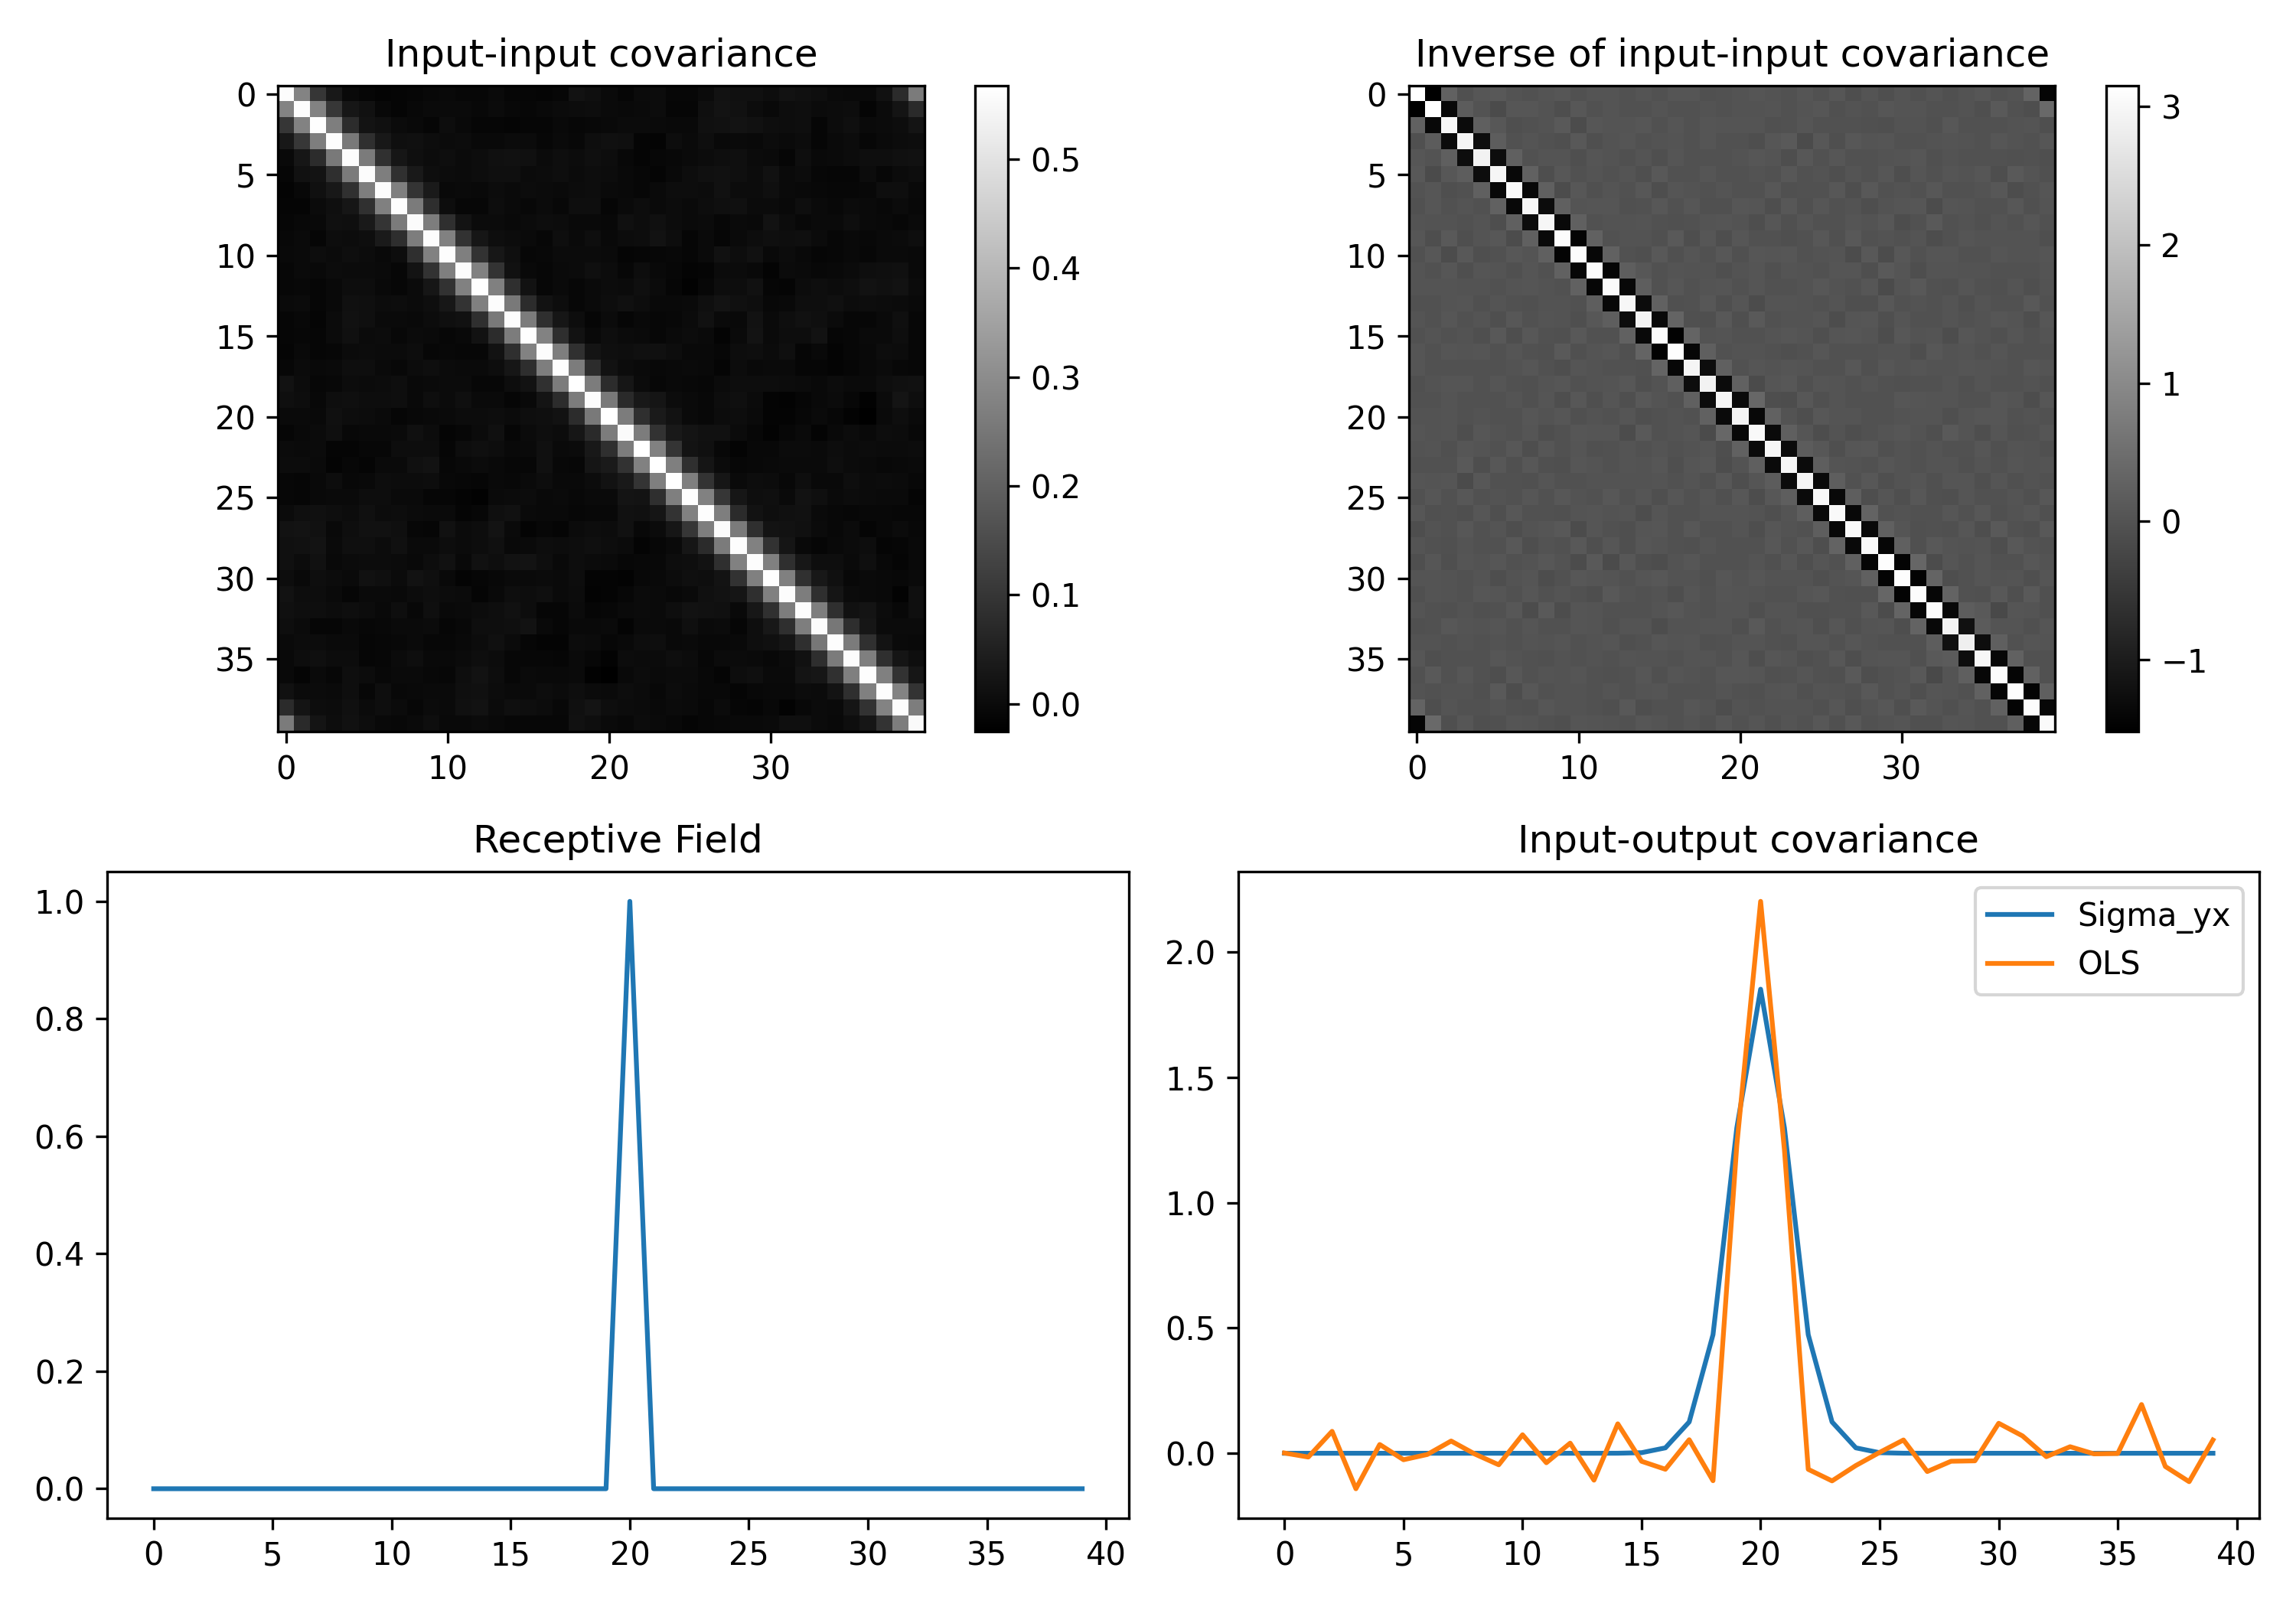
\includegraphics[width=0.45\textwidth]{../figs/math/OLS_small_bump.png} &
    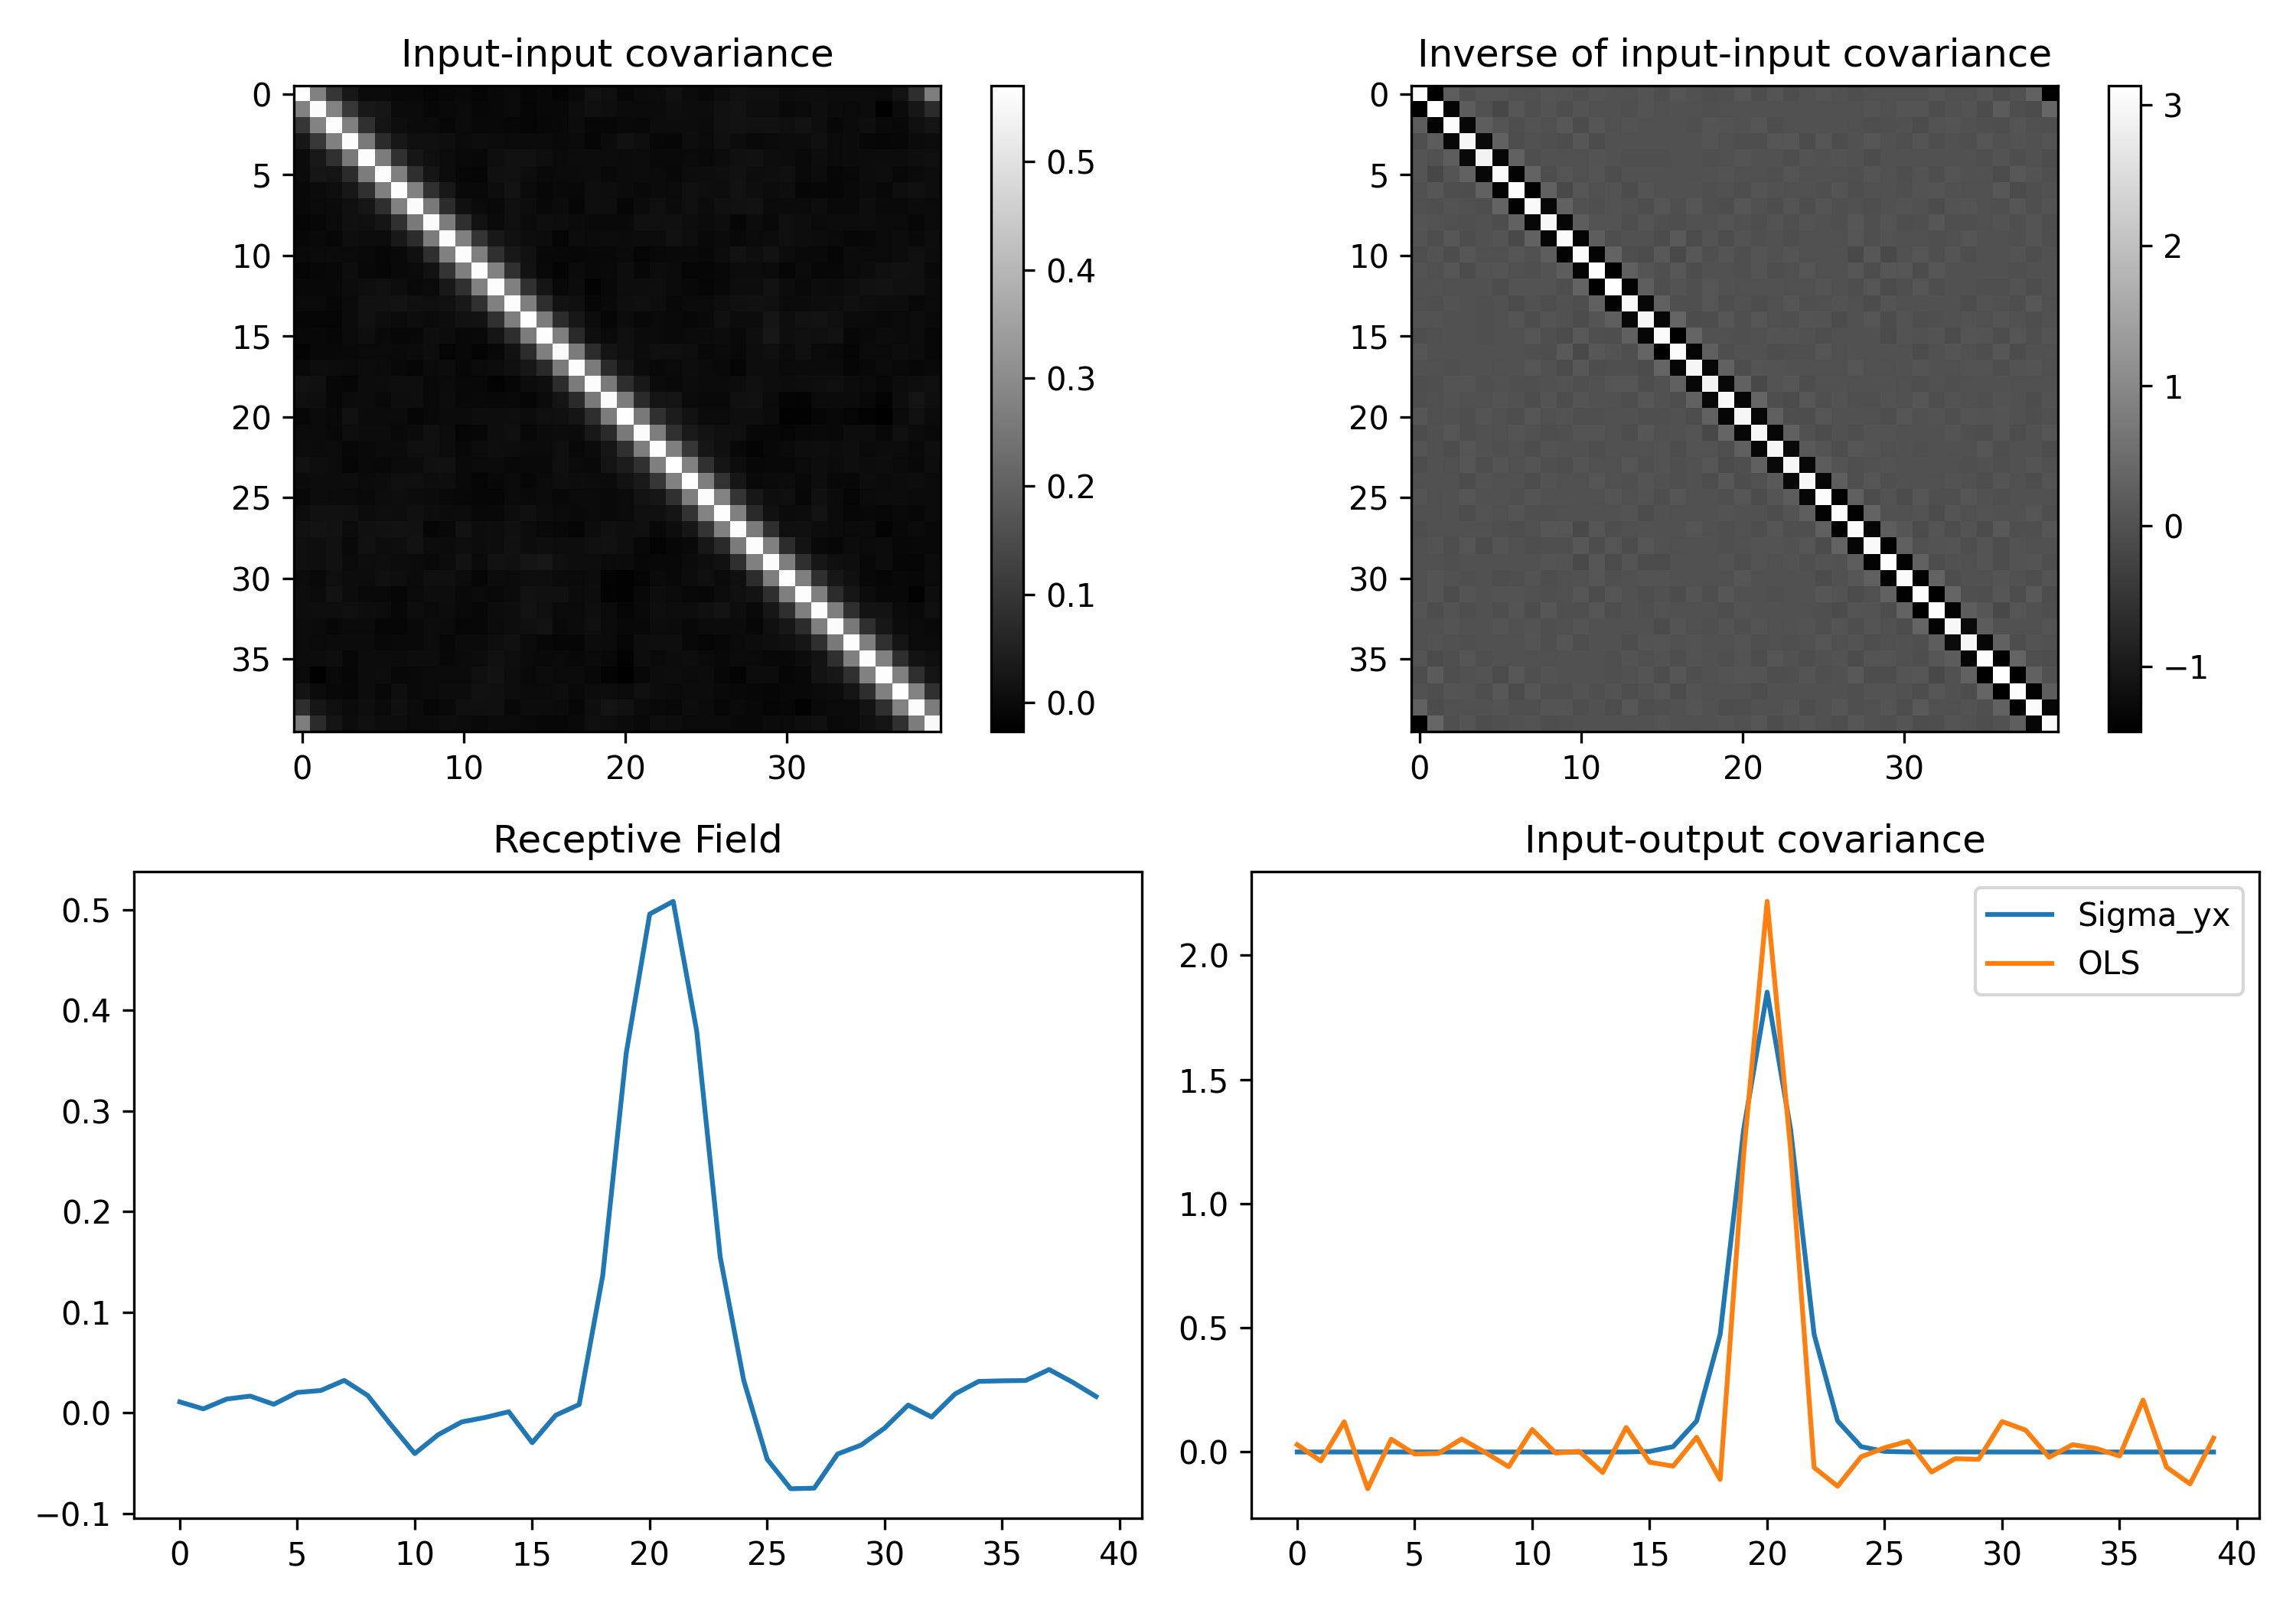
\includegraphics[width=0.45\textwidth]{../figs/math/OLS_mexican_hat.png} \\
    (a) & (b)
  \end{tabular}
  \caption{Input-input covariance, its inverse, the receptive field used to define the gate, and its effect on shaping $\Sigma^{yx}(p_i)$ to determine the OLS solution for (a) small-bump and (b) Mexican-hat-like receptive fields.}
  \label{fig:OLS}
\end{figure}


TODO: finish!



%%%%%%%%%%%%%%%%%%%%%%%%%%%%%%%
%% Stability of Localization %%
%%%%%%%%%%%%%%%%%%%%%%%%%%%%%%%
\section{Stability of Localization}

%%%%%%%%%%%%%%%%%%%%
%% Linear Pathway %%
\subsection{Linear Pathway}

%%%%%%%%%%%%%%%%%%%%%
%% Student-Teacher %%
\subsection{Student-Teacher}

%%%%%%%%%%%%%%%%%%%%%%%%%%%%%%%
%% Theory-driven Experiments %%
%%%%%%%%%%%%%%%%%%%%%%%%%%%%%%%
\section{Theory-driven Experiments}

\subsection{General Case}

\subsection{Single Gate}

\subsection{Redundant Gates}









\end{document}
